
% \newcommand{\DraftOrFinal}{draft}
\newcommand{\DraftOrFinal}{final}

\documentclass[\DraftOrFinal,11pt,letter]{article}

\newcommand{\DSU}{{\sc Jvolve}}
\newcommand{\transformObject}{\texttt{jvolve\_object}}
\newcommand{\transformClass}{\texttt{jvolve\_class}}
\newcommand{\VMClass}{\texttt{VM\_Class}}
\newcommand{\TIB}{\texttt{TIB}}
\newcommand{\JTOC}{\texttt{JTOC}}
\newcommand{\GroupC}{\suriya{Some name for Group C}}
\newcommand{\JikesRVM}{Jikes RVM}

\usepackage{acronym}
\usepackage{multirow}
\usepackage{epsfig}
\usepackage{fullpage}
\usepackage{float}
\usepackage{setspace}
\usepackage{url}
\usepackage{srcltx}
\usepackage[\DraftOrFinal,inline]{showlabels}
\usepackage{hyperref}
\usepackage{ifdraft}
\usepackage[usenames]{color}
\usepackage[override]{cmtt}
% \usepackage[centering,scale=0.80]{geometry}
% \usepackage{nopageno}
% \usepackage{array}

\ifdraft{
\newcommand\maybecolor[1]{\color{#1}}
\newcommand\mwh[1]{[{\maybecolor{red}\textbf{Mike says:} #1}]}
\newcommand\ksm[1]{[{\maybecolor{red}\textbf{Kathryn says:} #1}]}
\newcommand\suriya[1]{[{\maybecolor{blue}\textbf{Suriya says:} #1}]}
}{
\newcommand\mwh[1]{}
\newcommand\ksm[1]{}
\newcommand\suriya[1]{}
}

\begin{document}

\title{
       Dynamic Software Updates for Java:\\ A VM-Centric Approach\\
       \vspace{+0.5em}
       Ph.D. Proposal}

\author{Suriya Subramanian \\
        Department of Computer Sciences \\
        The University of Texas at Austin}

\date{July 21, 2008}

\maketitle

\subsection*{Abstract}
Software evolves to fix bugs and add features. Stopping and restarting
programs to apply changes is inconvenient and often costly.  Dynamic
software updating (DSU) addresses this problem by updating programs
while they execute, but existing DSU systems for managed languages do
not support many updates that occur in practice and are inefficient.
This paper presents the design and implementation of \DSU, a
DSU-enhanced Java VM.  Updated programs may add, delete, and replace fields
and methods anywhere within the class hierarchy.  \DSU{} implements
these updates by adding to and coordinating VM classloading,
just-in-time compilation, scheduling, return barriers, on-stack
replacement, and garbage collection.  \DSU{} is \emph{safe}: its use
of bytecode verification and VM thread synchronization ensures that an
% ISSUE: no bytecode verification in JikesRVM
update will always produce type-correct executions. \DSU{} is
\emph{flexible}: it can support 20 of 22 updates to three
open-source programs---Jetty web server, JavaEmailServer, and CrossFTP
server---based on actual releases occurring over 1 to 2 years.
%REFACTOR: though slight refactorings would allow the other updates.
\DSU{} is \emph{efficient}: performance experiments show that
\DSU{} incurs \emph{no overhead} during steady-state execution.  These
results demonstrate that this work is a significant step towards
practical support for 
dynamic updates in virtual machines for managed languages.

%%% Local Variables: 
%%% mode: latex
%%% TeX-master: "pldi64"
%%% End: 


% {
% \setbeamertemplate{headline}{}
% \setbeamertemplate{footline}{}
% \setbeamertemplate{navigation symbols}{}
% \begin{frame}
% \begin{block}{}
% \begin{quote}
% The only thing that is constant is change.\\
% \hfill Heraclitus of Ephesus
% \end{quote}
% \end{block}
% \end{frame}
% }

% \section{Introduction}
% \subsection{Motivation}
\begin{frame}{Motivation}%{A Sub-title is optional}
\begin{itemize}
\item Software applications change all the time
\item Deployed systems must be updated with bug fixes, new features
\item Updating typically involves: stop, apply patch, restart
% \vspace{1ex}
% \begin{center}\begin{Huge}Updating $\Rightarrow$ Downtime\end{Huge}\end{center}
\item Not desirable
  \begin{itemize}
    \item Safety concerns
    \item Revenue loss
    \item Inconvenience
  \end{itemize}
\end{itemize}
% \item Might not be affordable for some applications
%   \begin{itemize}
%   \item Applications that retain state that cannot be externalized
%   \end{itemize}
\end{frame}

\begin{frame}{Dynamic software updating}%{A Sub-title is optional}
\vspace*{-3mm}%
\begin{center}%
\includegraphics[scale=0.73]{images/process-state/both-process-state}%
\end{center}%
\end{frame}

\begin{frame}{Dynamic updating systems}%{A Sub-title is optional}
\begin{itemize}
\item Special-purpose architectures, application-specific solutions exist
\item General-purpose solutions gaining strength
  \begin{itemize}
  \item K42, Ksplice for OS updates
  \item Polus, Ginseng for C applications
  \end{itemize}
\item Not for managed languages
\end{itemize}
\end{frame}

% \begin{frame}{Motivation}%{A Sub-title is optional}
% \begin{itemize}
% \item Software applications change all the time
% \item Deployed systems need to be updated
% \item Some systems cannot afford downtime (safety concerns, revene loss),
% many systems perfer to avoid downtime (inconvenience)
% \item Stopping, updating and restarting deployed systems is not ideal
% \item Neither is delaying critical updates
% \end{itemize}
% \end{frame}

% \begin{frame}{Motivation}%{A Sub-title is optional}
% \begin{itemize}
% \item 75\% of downtime in high-availablity applications is for planned
% maintenance
% \uncover<2->{
% \item Personal operating system
% \item Enterprise applications
% \item Telecommunication, transportation systems
% % \uncover<3->{
% % \item Even a cache with lots of state
% %   \begin{itemize}
% %   \item LinkedIn.com architecture\footnote{\scriptsize{\url{http://hurvitz.org/blog/2008/06/linkedin-architecture}}}
% %   \item ``The Cloud'': In memory representation of the LinkedIn network graph
% %   \item Network size - 22M nodes, 120M edges
% %   \item Rebuilding an instance takes 8 hours
% %   \end{itemize}
% % }
% }
% \end{itemize}
% \end{frame}

% % \subsection{Solutions}
% \begin{frame}{Conventional solutions to avoid downtime}%{A Sub-title is optional}
% \begin{itemize}
% \item Move state out of the process, for instance databases
% \item Use multiple processes, and do a rolling update
% \end{itemize}
% \uncover<2>{
% \begin{itemize}
% \item Not always possible
% \item Restricted to specific application domains
% % \item DSU is a generic solution
% \end{itemize}
% }

% \begin{frame}{Dynamic Software Updating}%{A Sub-title is optional}
% Updating state of a process on the fly
% \begin{itemize}
% \item Special purpose techniques/architectures work, but we want a general
% solution
% \item 
% \end{itemize}
% \end{frame}

%   \begin{itemize}
%   \item State stored externally, for instance databases
%   \item Redundant systems: start a new process and stop this one
%   \item Not always possible
%   \end{itemize}
% \item<2-> Dynamic Software Updating (DSU)
%   \begin{itemize}
%     \item Update process state without restarting application
%     \item Non-redundant systems benefit as well
%     \item Decouples fault-tolerance from software updating
%   \end{itemize}
% \end{frame}

% \begin{frame}{Process state}%{A Sub-title is optional}
% \vspace*{-2ex}\includegraphics[scale=0.72]{images/process-state}
% \end{frame}

% \begin{frame}{DSU requirements}%{A Sub-title is optional}
% % \begin{center}
% % A Dynamic Software Updating solution should \emph{ideally} be
% % {\bf safe}, {\bf flexible}, and {\bf efficient}.
% % \end{center}
% \begin{description}
% \item[Safe] Updating is as correct as starting from scratch
% \item[Flexible] Support changes encountered in practice
% \item[Efficient] No performance impact
% \end{description}
% \end{frame}

% \begin{frame}{State of the art}%{A Sub-title is optional}
% Significant progress for C
% \begin{itemize}
% \item Server feature upgrades
%   \begin{itemize}
%   \item Ginseng \cite{neamtiu06dsu}
%   \item POLUS \cite{chen:icse07}
%   \end{itemize}
% \item Security patches: OPUS \cite{altekar05opus}
% \item Operating system upgrades
%   \begin{itemize}
%   \item K42 \cite{K42reconfig}
%   \item DynAMOS \cite{dynamos_eurosys_07}
%   \item LUCOS \cite{chen06vee}
%   \item Ksplice \cite{Ksplice}
%   \end{itemize}
% \end{itemize}
% % \item<2-> Primitive support for managed languages
% %   \begin{itemize}
% %   \item Very restrictive
% %   \item Space and time overheads
% %   \item Not proven on realistic applications
% %   \end{itemize}
% \end{frame}

% \begin{frame}{DSU opportunity for managed languages}%{A Sub-title is optional}
% DSU Solutions for C/C++ typically
% \begin{itemize}
% \item Require special compilation
% \item Statically/dynamically insert indirection for function calls
% \item Restrict structure updates, require extra allocation
% \item Impose space/time overheads on normal execution
% \item Make type-safety for updates difficult
% \item Not multi-threaded
% \end{itemize}
% \end{frame}

% \begin{frame}{Possible DSU solutions}%{A Sub-title is optional}
% Achieve DSU support by
% \begin{itemize}
% \item Making the application DSU-aware
% \item Special recompilation
% \item A class loader based colution 
% \item DSU support in the VM
% \end{itemize}
% \end{frame}

% \begin{frame}{Related work}%{A Sub-title is optional}
% \begin{itemize}
% \item Custom class loader solutions:\\Eisenbach and Barr, Milazzo et al.
% \item Source-to-source translation: Orso et al.
% \item VM-based solutions: JDrums, Dynamic Virtual Machine (DVM)
% \item In a persistent object store: Boyapati et al.
% \end{itemize}
% \uncover<2>{
% \begin{itemize}
% \item Limited, not flexible
% \item Restricted data-transformation model (like requiring {\em encapsulation} based
% on {\em ownership types})
% \item Overhead during normal execution
% \end{itemize}
% }
% \end{frame}

% \begin{frame}{Existing solutions for managed languages}%{A Sub-title is optional}
% \begin{itemize}
% \item VM-based solutions
%   \begin{itemize}
%   \item JDrums \cite{ritzau00dynamic}, DVM \cite{Mala00a}
%   \item Not well evaluated
%   \item Provide an interface similar to \DSU{}
%   \item Perform lazy updates
%   \item Overheads during normal execution
%   \end{itemize}
% \item Standard VM with DSU support
%   \begin{itemize}
%   \item DJVCS \cite{BarrE03}, DUSC \cite{orso:java}, \cite{Milazzo05updates}
%   \item Special classloaders, compilers
%   \item Very restrictive
%   \item Space/time overheads
%   \end{itemize}
% \end{itemize}
% 
% \end{frame}

% \begin{frame}{Related work}%{A Sub-title is optional}
% Nobody can beat us.
% \end{frame}

\begin{frame}{Our solution}%{A Sub-title is optional}
\begin{itemize}
\item \DSU{} - a Java Virtual Machine with DSU support
% \item Built on top of Jikes RVM, a Java-in-Java VM
\item Key insight: Extend existing VM services
%   \begin{itemize}
%   \item Classloading
%   \item Bytecode verification%\footnote{Jikes RVM does not have a bytecode verifier}
%   \item Thread synchronization
%   \item JIT Compilation
%   \item On-stack replacement
%   \item Garbage collection
%   \end{itemize}
\item No DSU-related overhead during normal execution
\item Support updates to real world applications
\begin{block}{}
\emph{Dynamic software updating in managed languages can be achieved in a
{\bf safe}, {\bf flexible} and {\bf efficient} manner by naturally extending existing VM
services.}
\end{block}

\begin{block}{}
\emph{DSU support should be a standard feature of future VMs.}
\end{block}
\end{itemize}
\end{frame}

% \begin{frame}{Contribution}%{A Sub-title is optional}
% \setbeamercovered{invisible}
% \begin{block}{}
% \emph{Dynamic software updating in managed languages can be achieved in a
% {\bf safe}, {\bf flexible} and {\bf efficient} manner by naturally extending existing VM
% services.}
% \end{block}
% 
% \begin{block}<2->{Corollary}
% \emph{DSU support should be a standard feature of future VMs.}
% \end{block}
% \end{frame}

\section{Related Work}
\label{sec:related}
We compare our VM-centric approach to DSU with related work on
implementing DSU for managed languages, C, and C++.

\paragraph{Edit and continue.}

Debuggers and IDEs have long provided \emph{edit and continue} (E\&C)
functionality that permits limited modifications to program state to
avoid stopping and restarting during debugging. For example, Sun's
HotSwap VM~\cite{JVMhotswap,Dmit01a}, .NET Visual Studio for C\# and
C++~\cite{VSEnC}, and library-based support~\cite{eaddy05enc} for .NET
applications all provide E\&C.  These systems restrict updates to
code changes within method bodies.  While this restriction reduces safety
concerns and obviates the need for class and object transformers, the resulting
systems are inflexible. They cannot perform more than half of the updates discussed in
Section~\ref{sec:experience}.

\paragraph{DSU for managed languages without VM support. } To avoid
changing the VM to support DSU, researchers have developed special-purpose
classloaders and/or compiler support.  The main drawbacks of these
approaches are inflexibility and high overhead.
For example, Eisenbach and Barr~\cite{BarrE03} and Milazzo et
al.~\cite{Milazzo05updates} use custom classloaders for
binary-compatible and component-level changes respectively, but
cannot perform class field additions.
% The former targets libraries and the latter is part of the design of a
% special-purpose software architecture.

%% Eisenbach and Barr: safe upgrading without restarting.  They support
%% upgrades that satisfy binary compatibility.  Uses a custom classloader and
%% JMX to replace the code of existing objects.  No way to modify the state of
%% the objects.

%% Milazzo use a modified class loader to load individual replacements to
%% classes in a special-purpose architecture.  The class loader may modify the
%% bytecode of the loaded class to deal with type version namespace issues.
%% Basically this is more limited in scope than our approach.

Orso et al.~\cite{orso:java} use source-to-source translation for DSU
by introducing a proxy object that indirectly accesses
an object that may change.  
%% For each class C that might change in the future they produce a proxy for
%% that class.  All calls from clients of C are redirected to call the wrapper
%% instead.  When C is updated by some new class C', a new C' object is created
%% and initialized using the old state of C and the wrapper is redirected to
%% point to C'.
This approach requires updated classes to export the same public
interface, forbidding new public methods and
fields.
Non VM-based approaches are in general limiting because they are
not \emph{transparent}---they make visible changes to the class hierarchy,
and insert or rename classes.  This approach makes it essentially
impossible to be robust in the face of code using reflection or native
methods.  Moreover, the indirection imposes time and space overheads
on steady-state execution.  Our VM approach
naturally supports reflection and native methods (these are updated
as well), and is more expressive, e.g., it supports signature changes.

\paragraph{VM support for DSU in managed languages.} 
The PROSE system performs short-term, run-time patches to code for
logging, introspection, and performance adaptation, rather performing
general updates~\cite{nicoara:eurosys08}.  An Eclipse plug-in performs
run-time bytecode instrumentation and a modified JIT performs method
code replacement, using an API in the style of aspect-oriented
programming.  % in support of run-time software
PROSE has the same update model as the E\&C systems: it supports updates to method bodies but not
class or method signature changes that require changes to object state. 
% This flexibility is
% similar to the EnC implementations discussed above; 
% indeed, PROSE builds on the HotSwap method replacement support in its
% Sun JDK implementation~\cite{JVMhotswap}.

JDrums~\cite{ritzau00dynamic} and Dynamic Virtual Machine
(DVM)~\cite{Mala00a} both implement DSU for Java within the VM,
providing a programming interface similar to \DSU, but are lacking in
two ways.  First, neither JDrums nor DVM have ever been demonstrated
to support updates from real-world applications.  Second,
their implementations impose overheads during steady-state execution.
They both update \emph{lazily} and use
an extra level of indirection (the \emph{handle
  space}).  Indirection conveniently supports
object updates, but adds extra overhead.  For example, JDrums traps
all object pointer dereferences to apply VM object transformer
function(s) when the object's class changes.  Lazy updating has the
advantage that it amortizes  pauses due to an update over
subsequent execution.  The main drawback is that its overhead persists
during normal execution, even though updates are relatively rare.  DVM
works only with the interpreter.  Relative to this interpreter, which
is already slow, the extra traps result in roughly 10\% overhead.

Compared to these two, \DSU{} performs updates eagerly by employing a
full heap collection at update-time.  This stop-the-world approach imposes a longer pause at
update time, but eliminates overhead during steady-state execution.
Likewise, by invalidating updated methods, \DSU's performance is
slowed just after the update as these methods are being recompiled.
However, compared to running with an interpreter, steady-state
execution is much improved, since methods will be much better
optimized.

%% JDRUMS: implements the conversion lazily.  They have a similar interface
%% (object and class transformers). The drawback here is that there is overhead
%% in the general case of execution---we do not know when the update is
%% complete.  Implemented in Sun's JDK 1.2.  Adds a level of indirection to the
%% new object.  Thus overhead builds up over time.  It also appears they have a
%% more limited interface to what can be referenced in a conversion function.
%% For example, there is no way to refer to fields other than those of the
%% object's class (i.e., no super-class fields) and there is no way to call new
%% methods, like constructors.  Not clear if there are restrictions on how
%% methods can be changed.

%% DVM: use an incremental mark-sweep collector, where mark phase marks objects
%% to be updated and the sweep phase incrementally updates them (prior to being
%% accessed by the mutator).  Like JDRUMS, all accesses to marked objects are
%% trapped.  Imposes a stock 10\% overhead, even only using bytecode.

%% Both of these: no significant experience with real applications, according
%% to how they change in practice.  They also can't handle native methods
%% because they can't trap access to modified objects.  Doing the full GC
%% solves this problem.

% More recently, Nicoara et al. developed PROSE, a system for run-time

Boyapati et al.~\cite{boyapati03lazy} support dynamic updates to
classes kept in a \emph{persistent object store} (POS).  While the
setting is different, their basic update model, and in particular
their notion of object transformer function, is similar to ours.  In
their system, programmers manually write an object transformer
that they view as a method on the old version of the updated class, i.e., the transformer method is type-safe with respect to the old class.
In \DSU, object transformers may access the \emph{new} versions of
objects pointed to from the old class.  Instead, Boyapati et al.'s
transformers may access the \emph{old} versions.  To implement this
model, they rely on
\emph{encapsulation} based on \emph{ownership types}: if an object $a$ of class $A$ has an ``owned''
field pointing to an object $b$ of class $B$, then only $a$ can point
to (and access) $b$.  Encapsulation thus ensures the system will always transform $a$ before $b$, which makes the transformation
algorithm more efficient.  They rely on the programmer to 
enforce encapsulation, and describe how the compiler could automate language support for encapsulation in a non-standard type system.  
\DSU{} takes the opposite tack of forcing old object fields to point
to up-to-date objects, and thus requires no special language support.
Moreover, \DSU's model follows that of earlier
work~\cite{k42usenix,neamtiu06dsu,neamtiu09stump,upstare} which has
proven its effectiveness on a half-dozen realistic applications
across several years' worth of releases.  However, further
research to understand the costs and benefits of the two updating
models would be useful.

Boyapati et al. also differs from \DSU{} in that, like JDRUMS and DVM,
updates are applied incrementally as objects are accessed following
an update rather than all at once using a stop-the-world GC\@.  This
incremental cost is more natural in a POS since indirection is
already required to access external objects.  The POS model also
permits programmers to specify ACID transaction boundaries, which can
help ensure that updates are applied consistently and safely.  In contrast, our work focuses on 
supporting dynamic upgrades in a high-performance VM for Java, and thus many of
the issues we consider---reaching a safe point via return barriers and
OSR, and coexisting with the JIT compiler---are the unique
contributions of our work.

% \paragraph*{Approaches using a standard VM.}
% \suriya{another
% awkward title. Should ask Kathryn what it actually is}
% 

\paragraph{Dynamic Software Updating for C/C++}

There are several substantial systems for dynamically updating C and
C++ programs that target server
applications~\cite{HjalmtyssonG98,altekar05opus,neamtiu06dsu,chen:icse07,upstare,neamtiu09stump}
and operating systems
components~\cite{K42reconfig,k42usenix,chen06vee,lee06linuxmod,dynamos_eurosys_07}.
% These systems are more mature than most of the systems described above, in
% some cases with substantial updating experience.  The flexibility
Although some of these systems are mature, the flexibility
afforded by \DSU{} is comparable or superior.  \DSU's timing
restrictions and Java's type safety also provide comparable or
superior safety; the fact that C and C++ programs often circumvent the
languages' weak type systems greatly complicates efforts 
to ensure that updates behave correctly.  Some prior
systems~\cite{neamtiu09stump,upstare,chen:icse07} have focused 
on means to reach DSU safe points quickly, and we plan similar
efforts as future work.  In particular, we plan to extend our support
for OSR to apply to running methods whose bytecode has changed,
allowing the user to map an active method's PC and
stack frame and those of its new version, similar to support provided by
UpStare~\cite{upstare}.

The lack of a VM is a disadvantage for C and C++ DSU.  For
example, because a VM-based JIT can compile and recompile replacement
classes, it imposes no steady-state execution overhead.  By contrast,
C and C++ implementations must use either statically-inserted
indirections~\cite{HjalmtyssonG98,neamtiu06dsu,K42reconfig,k42usenix,upstare}
or dynamically-inserted trampolines to redirect function
calls~\cite{altekar05opus,chen06vee,chen:icse07,ksplice}.  Both cases
impose persistent overhead on normal execution and inhibit
optimization.  Likewise, because these systems lack a garbage
collector, they either do not update object instances at
all~\cite{ksplice}, update them lazily~\cite{neamtiu06dsu,chen:icse07}
or perform extra allocation and bookkeeping to locate the
objects at update-time~\cite{k42usenix}.  Finally, because these
systems lack support for on-stack replacement, they must pre-compile
potentially long-running methods specially, so that they can be
updated while they run.   These techniques impose time and space overheads on
steady-state execution, and in some cases limit update flexibility.

\paragraph*{Other proposals}

Gilmore et al.~\cite{GilmoreKW97} propose DSU support for modules in
ML programs using a similar, but more restrictive programming interface
compared with \DSU{}.  They formalize an abstract machine for
implementing updates using a copying garbage collector.
Duggan~\cite{DBLP:journals/acta/Duggan05} also proposes dynamic
updates to ML programs, focusing on lazy updates to data type
definitions.  Neither approach was ever implemented.

UpgradeJ~\cite{bierman08upgradej} is an extension to
the Java language design supporting class upgrades, in two flavors:
\emph{revision upgrades}, which may modify method bodies, and
\emph{evolution upgrades}, which may add new methods and fields.
Programmers control the effects of upgrades using \emph{version
annotations}, introduced by Bierman et al.~\cite{BiermanHSS03} in
earlier work.  For 
example, the programmer may write \texttt{o = new 
Button[1=]()} to force \texttt{o} to always use version~1 methods,
while writing \texttt{p = new Button[1+]()} or \texttt{p = new
  Button[1++]()} allows \texttt{p} to be revised or evolved,
respectively.  UpgradeJ's update model is easier to implement than
\DSU's because it need not change existing object instances.  Of
course, the downside is a loss of flexibility.  Many of the updates to
our benchmark applications change field contents and layout.  UpgradeJ does not support these updates.  On the other hand,
evolution upgrades add power over simple method
body updates, and consequently enable more real-world updates to be
supported~\cite{tempero08upgradej}.  There is no implementation of
UpgradeJ.






%% basic swapping for single modules.


%%% Local Variables: 
%%% mode: latex
%%% TeX-master: "pldi64"
%%% End: 

%MWH: had to move this here to get it to show up on page 2
\begin{figure*}[t]
\begin{center}
\scalebox{.7}{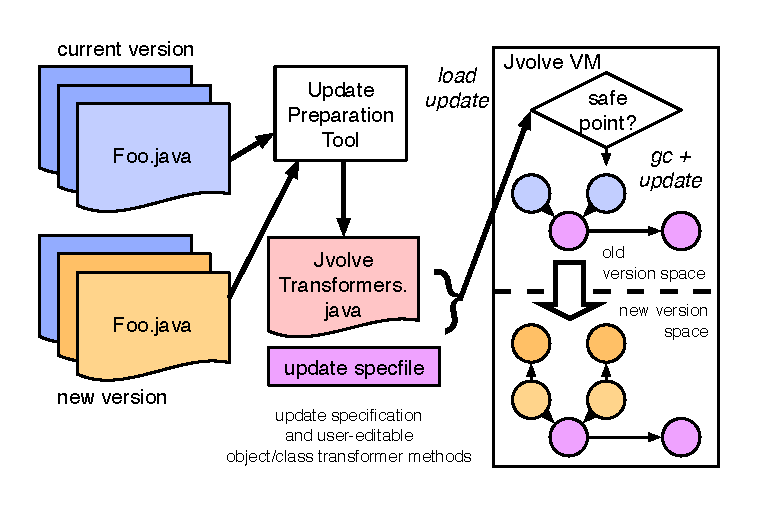
\includegraphics{system}}
\end{center}
\caption{Dynamic Software Updating with \DSU}
\label{fig:overview}
\end{figure*}



\section{Dynamic Updates in \DSU}

This section overviews how \DSU{} performs dynamic updating, including
the sorts of updates that \DSU{} supports, and how the developer
participates in the process.

%%  the developer responsibilities and how \DSU{}
%% performs updates.  We then summarize the simple update model that we
%% currently support.  Although simple, these updates are sufficient for
%% most of our test suite.  We postpone to Section~\ref{sec:saftey} our
%% discussion of the safety and flexibility implications of our simple
%% updates and of unsupported more sophisticated updates because they are
%% best understood once the VM collector and JIT support are explained in
%% Section~\ref{sec:VMdesign}.  Next, we give a running example to
%% help explain some of the issues with a VM based approach. 

\subsection{System Overview}

Figure~\ref{fig:overview} illustrates the dynamic update process.  It
shows the VM running the current version of the program and at top
left, the source files.  Meanwhile, developers are working on a new
version,
% \footnote{ Recent work in refactoring can help users prepare
%   their updates~\cite{HD:05}}
whose source files are shown at the
bottom left.  When the new version is ready--it compiles correctly and
the developer has fully tested it using standard procedures---the
developer passes the old and new versions of the source tree to \DSU's
\emph{change detector}.  This tool identifies classes that have
been added or changed and copies them into a separate directory.

At this point, the developer may write some number of \emph{object}
and \emph{class transformers}.
Transformer methods take an object or class of the old version and
produce an object or class of the new version.  For example, if an
update to class \texttt{Foo} adds a new instance field \texttt{x} and
a new \texttt{static} field \texttt{y}, the programmer can write an
object transformer (called \texttt{jvolve\_object}) to initialize
\texttt{x} for each updated object, and a class transformer (called
\texttt{jvolve\_class}) to initialize \texttt{y}.  If the programmer
chooses not to write one of these transformers, the system will
dynamically produce a default one that simply initializes each new field to its
default value and copies over the values of any old fields that have
not changed type.  Transformer methods are the only portions of code
where both views of the class definition are visible and they are only
ever invoked at update time.  This feature enables the programmer to
develop the application largely oblivious to the fact that it will be
dynamically updated.

%% The user compiles $v_1$ with \textsf{javac}, or
%% another Java to bytecode compiler, which guarantees that the update is
%% free from type, syntactic, and other errors.  For example, if the
%% update modifies a method signature, the update is guaranteed to
%% contain the updated versions of any class file that invokes the
%% method.

\DSU{} then translates the transformer functions to class files, which
ensures (among other things) that they are type correct.  The running
VM then starts the updating process by loading the transformers and the new
user class files.
% The first step is for the VM's JIT compiler to
% compile the loaded classes. 
  Next, the VM waits for all the threads to
stop at a DSU \emph{safe point}~\cite{HicksNettles03,neamtiu06dsu}
where none of their activation stack's
contain \emph{updated methods}. Updated methods include all the
directly updated methods and any methods that depend on them or
updated classes, e.g., due to inlining. Section~\ref{sec:safe}
describes some additional restrictions on safe points.  

The VM then adds any new entries to the method dispatch table, 
and invalidates any updated method implementations.  Changed methods
are then compiled as 
a matter of course the next time the program invokes them (and the old
implementations can never be accessed).  Finally,
the VM initiates a full copying garbage collection to update the state
of existing objects whose classes changed.  When the collector
encounters an object to update in the \emph{from space}, it allocates a copy
of this object and an object of the new class in the \emph{to space}. At the
end of the collection, \DSU{} runs object transformers on
each of these pairs and then invokes the class transformers.
At this point, the update is complete.

% Taken from outline.txt
% Section 2: Updating model (look at Dynamic ML paper section 2 for guidance)
%  Workflow
%    Show picture of the process
%      Develop patches
%      Compile them, ensure type correctness
%      Load 'em via classloading
%      Wait for the threads to reach a safe point, stop them, run GC
%        Intuitively discuss safe point condition; elaborate later
%      restart and resume (now the new version)

\subsection{Update Model}
\label{sec:updates}

We have designed a
flexible, yet simple update model that supports updates that we
believe are important in practice.  \DSU{} classifies updates into the
following two categories:

\begin{description}

\item[Method body updates:] These updates change just the internal
implementation of a method.
  
\item[Class updates:] These updates change the class signature by adding
or removing fields and methods, or by changing the signature of fields and
methods in a class.

\end{description}

\noindent 
Method body updates are the simplest and most commonly supported
updates~\cite{JVMhotswap,VSEnC,eaddy05enc,GilmoreKW97,orso:java,K42reconfig,HjalmtyssonG98},
because these changes do not require DSU safe points; they can be
applied at any time and preserve type safety.
Permitting only method implementation updates however prevents many
common changes~\cite{neamtiu05evolution}.  For example,
Section~\ref{sec:experience} shows that over half of the updates to
Jetty, JavaEmailServer and CrossFTP add fields and/or change
method signatures.

\begin{figure*}[t]
\begin{tabular}{c|c}
\begin{minipage}{3in}
\begin{footnotesize}
\begin{verbatim}
public class User {
  private String username, domain, password;
  private String[] forwardAddresses;
  public String[]
   getForwardedAddresses() {...}
  public void
   setForwardedAddresses(String[] f) {...}
}
public class ConfigurationManager {
  private User loadUser(...) {
     ...
     User user = new User(...);
     String[] f = ...;
     user.setForwardedAddresses(f);
     return user;
  }
}
\end{verbatim}
\end{footnotesize}
\end{minipage} &
\begin{minipage}{3.15in}
\begin{footnotesize}
\begin{verbatim}
public class User {
  private String username, domain, password;
  private EmailAddress[] forwardAddresses;
  public EmailAddress[]
   getForwardedAddresses() {...}
  public void
   setForwardedAddresses(EmailAddress[] f) {...}
}
public class ConfigurationManager {
  private User loadUser(...) {
     ...
     User user = new User(...);
     EmailAddress[] f = ...;
     user.setForwardedAddresses(f);
     return user;
  }
}
\end{verbatim}
\end{footnotesize}
\end{minipage} \\
(a) Version 1.3.1 &
(b) Version 1.3.2 \\
\end{tabular}
\caption{Example changes to JavaEmailServer \texttt{User} and
  \texttt{ConfigurationManager} classes}
\label{fig:email-example}
\end{figure*}


Class updates may occur at any level of the class hierarchy.  For
example, an update that deletes a field from a parent class will
propagate correctly to the class's descendants. Henkel et al.'s recent work in
refactoring ~\cite{Fowler,HD:05} categorizes changes into the following: renamed
types, moved Java elements, moved static members, changed method
signatures, renamed non-virtual methods, renamed virtual methods, renamed
fields, and generalization where occurrences of a type are replaced by a
particular super-type. \DSU{} supports all these changes.
\DSU{} does not support permutations of the class hierarchy, e.g.,
reversing a super-class relationship.  While this update may be desirable
in principle, in practice, it requires sophisticated transformers that can
enforce update ordering constraints. None of the program versions we
observed made this type of update.
% there are two problems.  First, it may be quite
% challenging to actually implement this change---the process of
% transforming old objects from the old to the new class hierarchy is
% complex.  Second, complex changes make it harder to reason that an
% update's semantics will be correct.  To see why, consider that a
% common limitation of existing code updating systems is that they
% support only method body updates, not method signature
% updates~\cite{JVMhotswap,VSEnC,eaddy05enc,GilmoreKW97,orso:java,K42reconfig,HjalmtyssonG98}.
% The reason is that such changes can take effect at any time and
% preserve type safety, whereas changes to method signatures must take
% timing into account.  However, permitting only method implementation
% updates prevents many common changes~\cite{neamtiu05evolution}
% including the example in Figure~\ref{fig:email-example}.  Therefore,
% any practical system must trade off flexibility with
% availability---the more flexible the update, the greater burden on the
% system to ensure that updates are well-timed.
\DSU's update model is quite flexible.  Developers may change a method
implementation to fix a bug.  Developers may enhance functionality by
adding and acting on a new parameter to a method, or by adding a new
field and its access methods to a class (and its subclasses, as desired).
% \DSU's supported updates also match common refactorings, such
% as dividing a method into multiple methods, renaming a class or
% interface, changing types, and renaming fields~\cite{Fowler}.
% Sections~\ref{sec:safe} and~\ref{sec:xformers} provide additional
% details on the safety, flexibility, and implementation of our
% update model and possible enhancements.
Currently, \DSU{} does not
allow classes with such changes as described above to have active methods
on stack when performing the update. We propose to extend \acf{OSR},
as described in section~\ref{sec:safe} can help remove this restriction.

\paragraph{Example.} 
Consider the following update from JavaEmailServer, a simple SMTP and
POP e-mail server.  Figure~\ref{fig:email-example}
illustrates a 
pair of classes that change between versions 1.3.1 and 1.3.2.  These
changes are fully supported by \DSU.  JavaEmailServer uses the class
\texttt{User} to maintain information about e-mail user accounts in the
server.  Moving from version 1.3.1 to 1.3.2, there are two
differences.  First, the method \texttt{loadUser} fixes some problems
with the loading of forwarded addresses from a configuration file
(details not shown).  This change is a simple method update.  Second,
forwarded addresses are represented as an array of instances of a new
class, \texttt{EmailAddress}, rather than \texttt{String}.  This change modifies
the class signature of \texttt{User} since it modifies the type of
\texttt{forwardedAddresses}.  The class's
\texttt{setForwardedAddresses} method is also altered to take an array of
\texttt{EmailAddress}es instead of an array of \texttt{String}s.


\subsection{Class and Object Transformers}
\label{subsec:transformers}

For our example, the \DSU{} change detector  identifies that
the \texttt{User} and \texttt{ConfigurationManager} classes have
changed.  At this point, the programmer may elect to write object
and class transformers or use the defaults.
The user elects to write both a class and object
transformer for the class \texttt{User}, as illustrated in
Figure~\ref{fig:example-xform}.

Object and class transformer methods are simply \texttt{static}
methods that augment the new class.  The class transformer method
\texttt{jvolve\_class} (body not shown) takes no arguments, while the
object transformer method \texttt{jvolve\_object} takes two reference
arguments: \texttt{to}, the uninitialized new version of the object,
and \texttt{from}, the old version of the object.  For both methods,
the old version of the changed class has its version number prepended to its
name.  In our example, the old version of \texttt{User} is redefined as
class \texttt{v\_1\_3\_1\_User}, which is the type of the \texttt{from}
argument to the \texttt{jvolve\_object} method in the new \texttt{User}
class. The \texttt{v\_1\_3\_1\_User} class contains only field definitions
from the original class, defined with access modifier \texttt{public} to
allow them to be accessed from the \texttt{jvolve\_object} method.

The code in transformer methods is essentially a kind of constructor:
it should initialize all of the fields of the new class/object.  Very
often the best choice is to initialize a new field to its default
value (e.g., \texttt{0} for integers or \texttt{null} for references)
or to copy references from the old values.  In the example, the first
few lines simply copy \texttt{username}, \texttt{domain}, and other
fields from their previous values.  A more interesting case is the
field type change to \texttt{forwardedAddresses}. % the user
% initializes the new field by referring to the old field.  The
The
function allocates a new array of \texttt{EmailAddress}es
initialized using the \texttt{String}s from the old array.  Note that
the default transformer function would instead copy the first three
fields as shown, and initialize the \texttt{forwardedAddresses} field
to \texttt{null} because it has changed type.

Supported in its full generality, a transformer method may
reference any object reachable from the global (\texttt{static})
namespace of both the old and new classes, and read or write fields or
call methods on the old version of the object being updated and/or any
objects reachable from it.  \DSU{} presents a more limited interface
similar to that of past work~\cite{ritzau00dynamic,Mala00a}.  In
particular, transformers may only use old objects to initialize new
objects; the only safe access to a new object is through the
\texttt{to} argument.  Transformers may safely copy the contents of
\texttt{from} fields.  These fields may also be dereferenced if the
update has not changed their class, or if it has, after
the referenced objects are transformed to conform to the new class
definition.  \suriya{Clarify the next sentence} At the moment this is achieved by invoking a VM function,
but ultimately we plan to provide more automatic support.
Finally, object transformers may not call methods
on the old object. For example in Figure~\ref{fig:example-xform},
class \texttt{v\_1\_3\_1\_User} is defined in terms of the fields it
contains, \suriya{clarify} while the methods have been removed.  As explained in
Section~\ref{sec:xformers}, these limitations stem from a goal to keep
our garbage collector-based traversal safe and relatively simple.
This interface is sufficient to handle all of the updates we tested, but
other programs may require a more flexible approach. \suriya{so? is this
true?}

\begin{figure}
\begin{small}
\begin{verbatim}
public class v_1_3_1_User {
  public String username, domain, password;
  public String[] forwardAddresses;
}
public class User {
 ...
 public static void jvolve_class() { ... }
 public static void 
  jvolve_object(User to, v_1_3_1_User from) {
    to.username = from.username;
    to.domain = from.domain;
    to.password = from.password;
    // default transformer would have:
    //   to.forwardAddresses = null
    int l = from.forwardAddresses.length;
    to.forwardAddresses = new EmailAddress[l];
    for (int i = 0; i < l; i++) {
      to.forwardAddresses[i] = 
       new EmailAddress(from.forwardAddresses[i]);
}}}
\end{verbatim}
\end{small}
\caption{Example \texttt{User} object transformer}
\label{fig:example-xform}
\end{figure}

If a programmer does not write an object transformer, the VM % merely
initializes new or changed fields to their default values and copies the
values from unchanged fields. \DSU{}'s \ac{UPT} (described in
Section~\ref{sec:prep}) generates
\suriya{inconsistent with the first sentence of
section~\ref{subsec:transformers}}
default versions of the \texttt{jvolve\_object} and
\texttt{jvolve\_class} methods in the same way, which the user may
modify.


%% will have been verified to be type-correct by the Java-to-bytecode
%% compiler. In addition, \DSU{} has to appropriately handle
%% \verb|ConfigurationManager.loadUser|. \suriya{Should we say, we do not allow
%%   it to be on stack}.

%    Show the parts that change
%    Show the state transformer you would write

%  What is the API for the programmer?
%    Off-line patch tool to figure out what methods changed, etc.
%      (programmer doesn't have to worry about this)
%    State transformer as a method of the new class
%      - but only called during the update process
%      - namespace set up to be clear about which object versions
%        you are referring to




%% \subsubsection{Update Form}


%% To allow dynamic updates, \DSU{} must handle these two important types
%% of updates. (a) Changes within a body of a method that do not change
%% the class definitions type system. (b) Changes to the type system,
%% such as addition of fields, and method signatures.

%% (a) After an update, existing code must call the updated version of a
%% method. \DSU{} accomplishes this trivially by using the capabilities of the
%% JVM to recompile the method with its updated version. \DSU{} updates the
%% function indirection tables (the JTOC for static methods and TIB for
%% virtual methods) to point to the new version. This is similar to what
%% happens with JIT compilation of a method.

%% (b) A type T changes as a result of changes to its fields, or method
%% signatures. \DSU{} enforces \emph{representation consistency}
%% \cite{Stoyle-POPL-2005} in which all objects of type T must logically be of
%% type T's latest version. (This is almost copied from Ginseng. What should
%% we do?)

%% \DSU{} supports representation consistency by ensuring that when type T is
%% updated, all objects of that type in the running program are updated to
%% correspond to the new version. For each object of type T, \DSU{} calls a
%% state transformation function $c_{T_{n->n+1}}$ that converts an object
%% $o_T$ of type $T_n$ to one of type $T_{n+1}$. The type transformation
%% function is generated trivially for most updates, by comparing the old and
%% new definitions of a type.


\newcommand{\JvolveTimeLine}[5]{
\begin{center}
\begin{tikzpicture}[auto]
  \tikzstyle{block}=[
    font=\tiny,
    rectangle,
    draw=structure.fg,
    thick,
    text width=1.2cm,
    text badly centered,
    rounded corners,
    minimum height=2em,
  ]
  \tikzstyle{current}=[fill=structure.fg!20, ]
  \tikzstyle{line}=[draw, thick, -latex',]
  \tikzstyle{every path}=[line]
  \matrix [column sep=5mm,row sep=7mm,ampersand replacement=\&] {
    \node [block,#1] (0) {\hyperlink{offline}{Offline tool}};          \&
    \node [block,#2] (1) {\hyperlink{suspend}{Suspend application}};   \&
    \node [block,#3] (2) {\hyperlink{classload}{Install new classes}}; \&
    \node [block,#4] (3) {\hyperlink{transform}{Transform objects}};   \&
    \node [block,#5] (4) {Resume application};                         \\
  };
  \path (0) -- (1);
  \path (1) -- (2);
  \path (2) -- (3);
  \path (3) -- (4);
\end{tikzpicture}
\end{center}
}


\subsection{Implementation}
\ShowTOC

\begin{frame}{Update model}%{A Sub-title is optional}
\begin{itemize}
\item Update happens in one fell swoop
\item Simple to reason about
\item Code
  \begin{itemize}
  \item Old code before the update
  \item New code after the update
  \end{itemize}
\item Data
  \begin{itemize}
  \item Representation consistency (all values of a type correspond to the
        latest version)
  \item Support a transformation function to convert objects to the new
        type
  \end{itemize}
\end{itemize}
\end{frame}

\begin{frame}[t,fragile]{Update process}%{A Sub-title is optional}
\JvolveTimeLine{}{}{}{}{}
\begin{itemize}
\item Offline Update Preparation Tool (UPT)
\item \DSU{} VM
  \begin{itemize}
  \item Reach a safe point in the VM (thread synchronization)
  \item Load new classes (classloader)
  \item Transform objects to new definition (garbage collector)
  \item Resume execution
  \item<2-> Update active methods on stack (On-stack replacement)
  \end{itemize}
\end{itemize}
\end{frame}

\begin{frame}[t,fragile,label=offline]{Update Preparation Tool}%{A Sub-title is optional}
\vspace{-2ex}
\JvolveTimeLine{current}{}{}{}{}
\vspace{-2ex}
\begin{itemize}
\item Uses jclasslib\footnote{\url{http://jclasslib.sourceforge.net}}, a
bytecode library
\item Compares bytecode of the two versions
\item Categorizes changes into
  \begin{description}
  \item[Class updates] Classes that add, remove, change signature of fields
                       or methods
  \item[Method updates] Changes within a method body. Only the method has
                        to be loaded/updated
  \item[Indirect updates] No change to method, but refers to changed
                          classes
  \end{description}
\item Generates old version stubs and default object transformers
\end{itemize}
\end{frame}

\begin{frame}[t,fragile,label=suspend]{Safe point for the update}%{A Sub-title is optional}
\JvolveTimeLine{}{current}{}{}{}
\begin{itemize}
\item Update must be atomic
\item Updates happen at ``safe points'' (VM yield points with restriction
      on what methods can be on stack)
\item Uses a simple, non-deterministic timer retry
\item<2-> Supported only on a single processor
\item<2-> On-stack replacement support to allow more methods to remain on
          stack
\end{itemize}
\end{frame}

\begin{frame}[t,fragile]{Restricted methods}%{A Sub-title is optional}
\JvolveTimeLine{}{current}{}{}{}
\begin{itemize}
\item Identified by UPT
  \begin{itemize}
  \item All methods in updated classes
  \item Methods with new implementations
  \item Methods that refer to updated classes (have to be recompiled since
        field/method offsets might have changed)
  \end{itemize}
\item Identified by the VM
  \begin{itemize}
  \item With inlining, transitive closure of callers of methods identified
        above
  \end{itemize}
\end{itemize}
\end{frame}

{
\setbeamercovered{invisible}
\begin{frame}[t,fragile,label=classload]{Loading new classes}%{A Sub-title is optional}
\JvolveTimeLine{}{}{current}{}{}
\begin{itemize}
\item Modifications to the classloader
\item Involved a lot of engineering effort
\item<2-> Correctly update metadata maintained by the VM
  \begin{itemize}
  \item Classes
  \item Type information blocks
  \item Methods
  \item Fields
  \item Subclass, superclass relations
  \item Innerclasses
  \item Exceptions
  \item Annotations
  \end{itemize}
\end{itemize}
\end{frame}
}

\begin{frame}{VM Datastructures}%{A Sub-title is optional}
\begin{center}
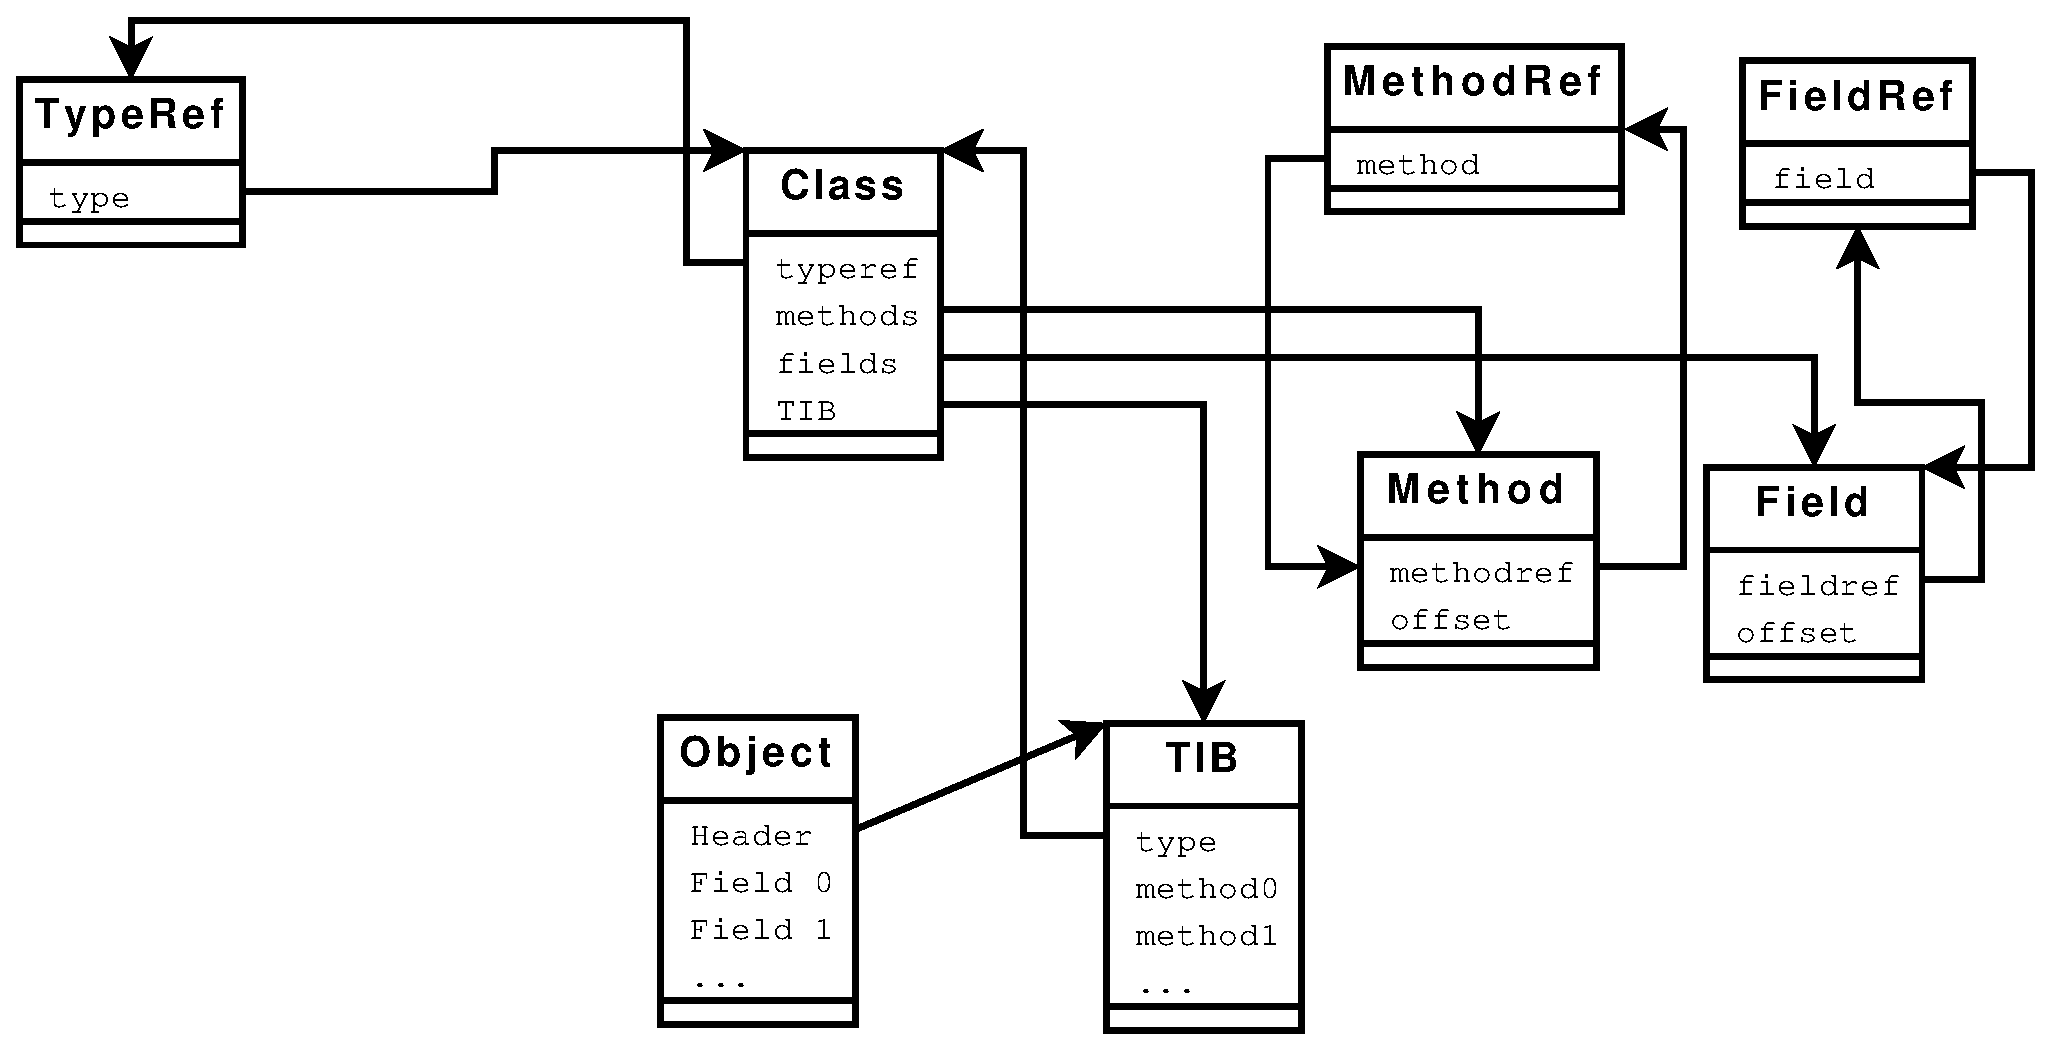
\includegraphics[width=0.84\paperwidth]{jvolve/vm-datastructures}
\end{center}
\end{frame}

\begin{frame}{VM Datastructures}%{A Sub-title is optional}
\begin{center}
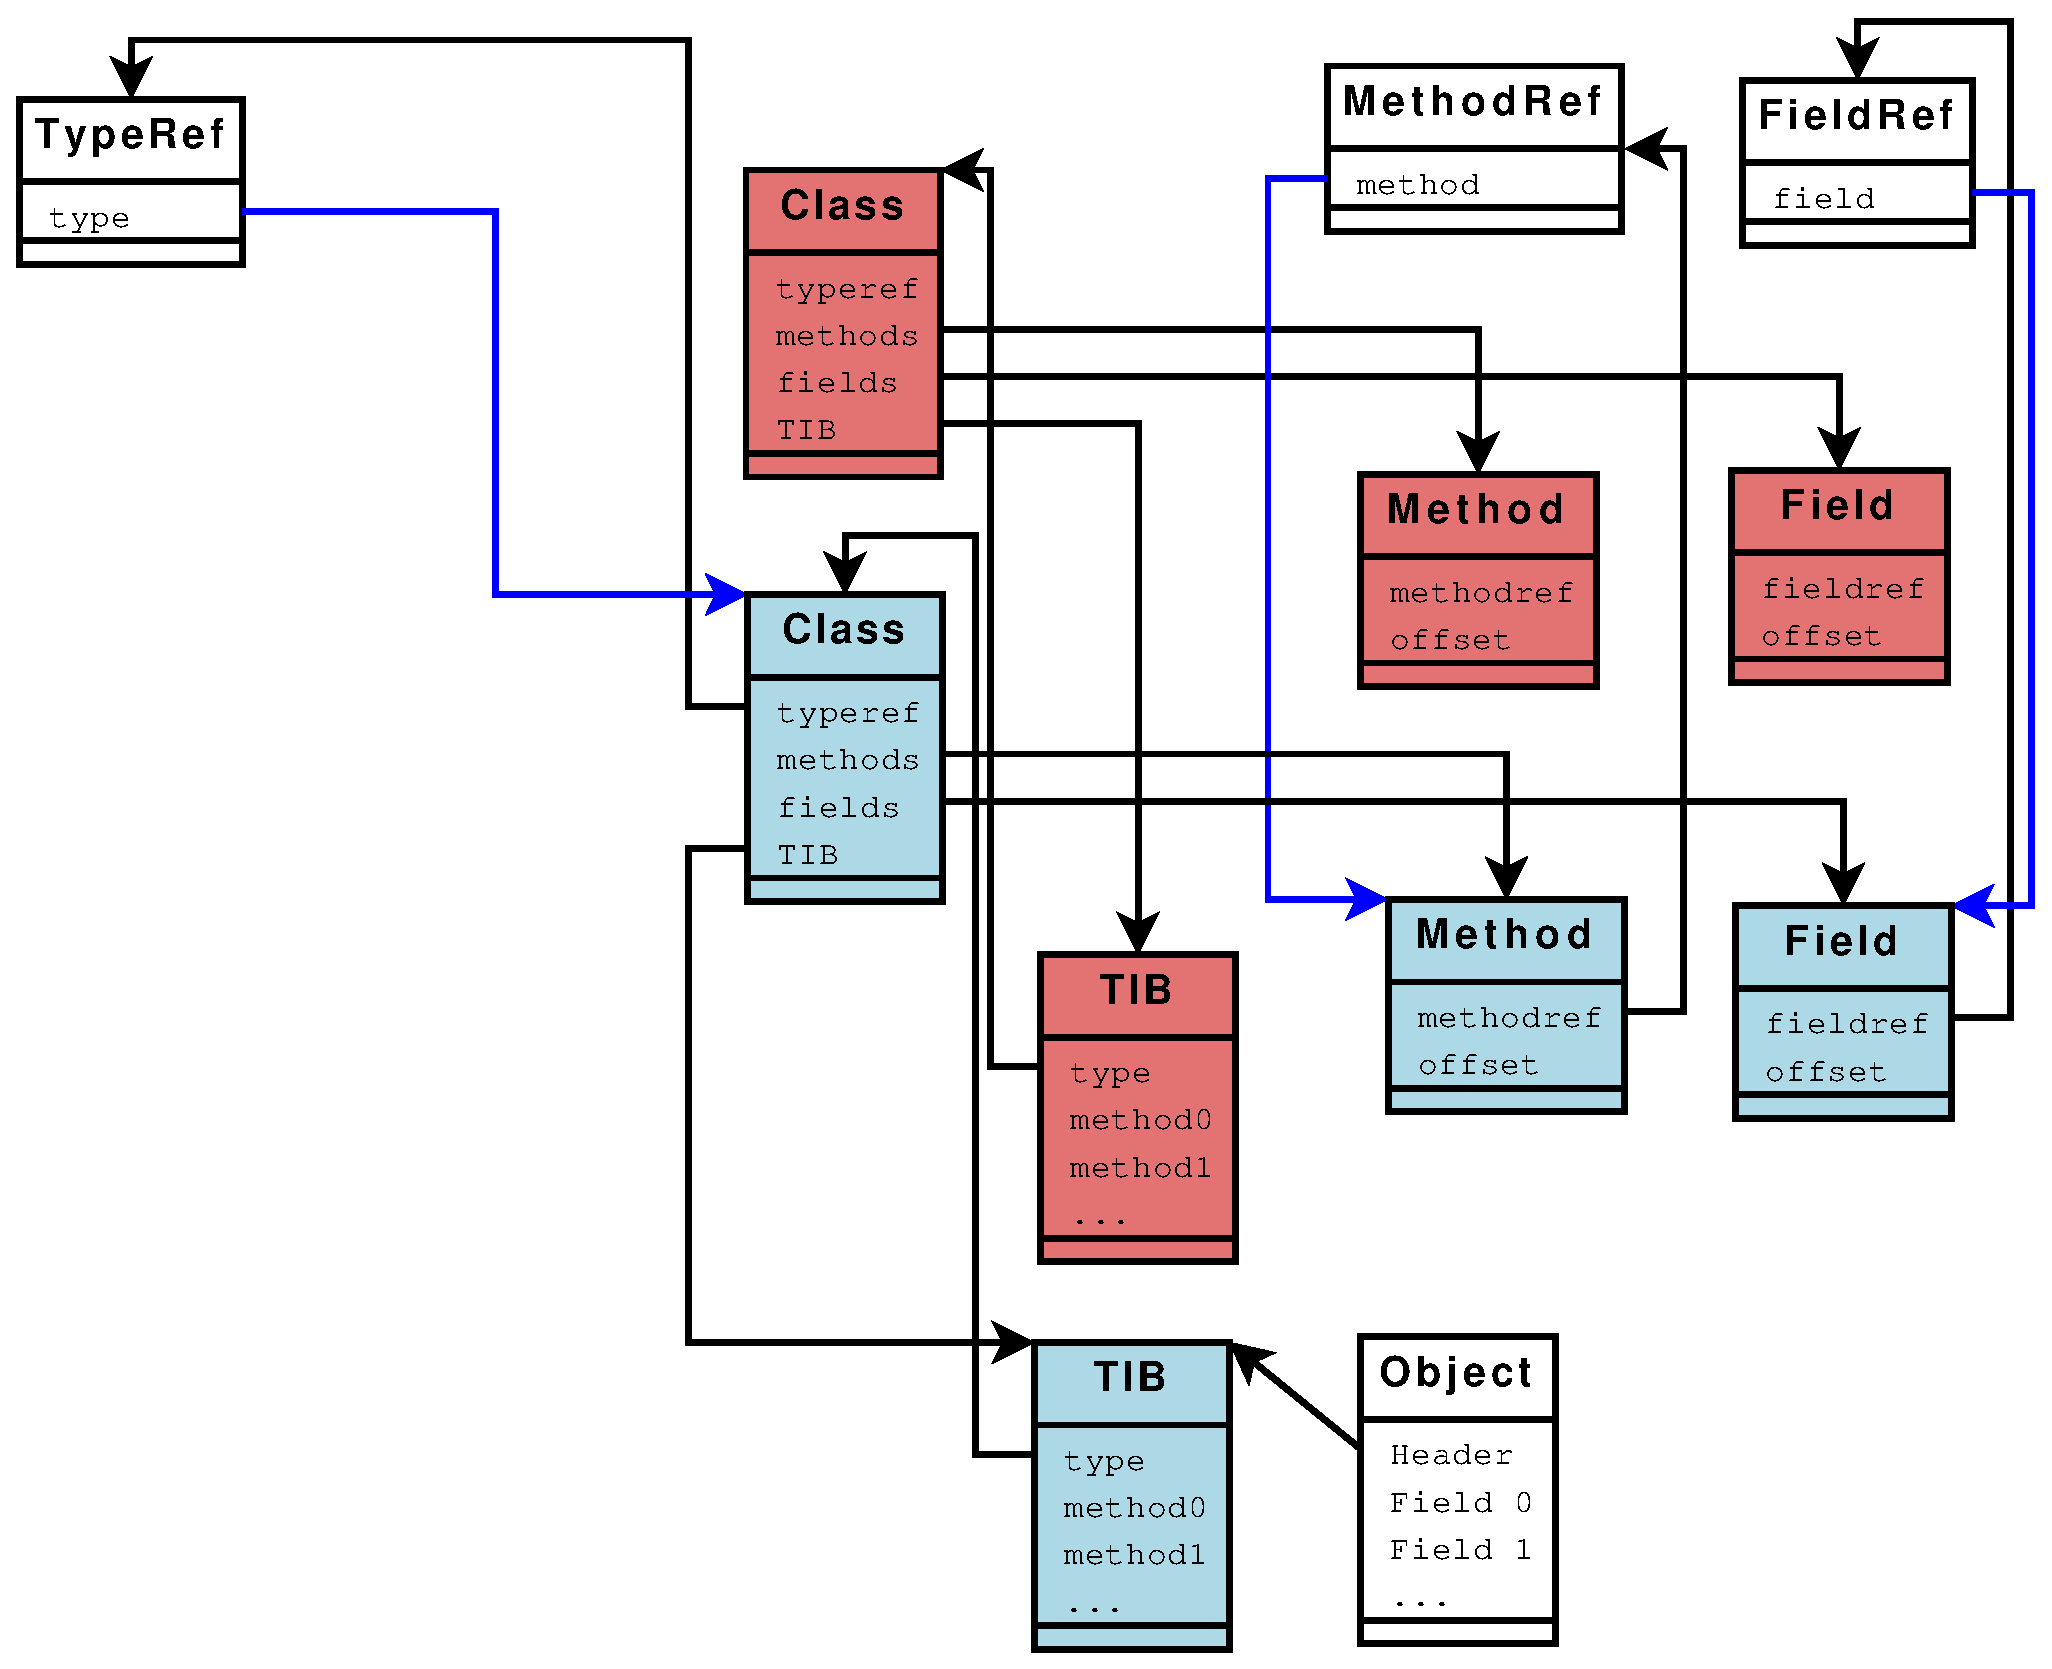
\includegraphics[width=0.84\paperwidth,height=0.7\paperheight]{jvolve/vm-datastructures-after-dsu}
\end{center}
\end{frame}

% \begin{frame}[fragile]{FXIME: Hierarchy}%{A Sub-title is optional}
% \begin{tikzpicture}
% \tikzstyle{every node}=[font=\scriptsize,circle,draw,minimum size=0.7cm]
% \tikzstyle{dsu node}=[every node,fill=structure.fg!50]
% \node at (0,0) (root) {A}
%   child {node {B}}
%   child {node[dsu node] {C}
%           child {node {D}}
%           child {node {E}}};
% \tikzstyle{level 1}=[sibling distance=3cm]
% \tikzstyle{level 2}=[sibling distance=2cm]
% \tikzstyle{level 3}=[sibling distance=1cm]
% \node at (6,0) {A}
%                       child {node {B}}
%                       child {node {C}
%                               child {node {D}}
%                               child {node {E}}}
%          child {node {Cx}
%                               child {node {Dx}}
%                               child {node {Ex}}}
%                      ;
% \end{tikzpicture}
% \end{frame}

\begin{frame}[t,fragile,label=transform]{Transforming objects}%{A Sub-title is optional}
\JvolveTimeLine{}{}{}{current}{}
\begin{itemize}
\item Built on top of a semi-space copying collector
\item Allocate additional space and run object transformers as part of the
      collector's visit
\end{itemize}
\end{frame}

\ifdraft{}{

%%%%%%%%%%%%%%%%%%%%%%%%%%%%%%%%%%%%%%%%%%%%%%%%%%%%%%%%%%%%%%%%%%%%%%%%
% Colors
\colorlet{black object color}{black!60}
\colorlet{grey object color}{black!20}
\colorlet{forwarding pointer color}{structure.fg!40}
\colorlet{dsu v0 color}{blue!60}
\colorlet{dsu v1 empty color}{blue!20}
\colorlet{dsu forwarding pointer color}{forwarding pointer color!50!dsu v0 color}
%%%%%%%%%%%%%%%%%%%%%%%%%%%%%%%%%%%%%%%%%%%%%%%%%%%%%%%%%%%%%%%%%%%%%%%%

%%%%%%%%%%%%%%%%%%%%%%%%%%%%%%%%%%%%%%%%%%%%%%%%%%%%%%%%%%%%%%%%%%%%%%%%
% Define the style for each field of the object
\newlength{\drawthickness}
\setlength{\drawthickness}{0.6pt}
\newlength{\fielddimension}
\setlength{\fielddimension}{5mm}
\tikzstyle{field}=[
    rectangle,
    draw=black,
    line width=\drawthickness,
    minimum width=\fielddimension,
    minimum height=\fielddimension,
    inner sep=0pt,
    font=\tiny,
]
\tikzstyle{new space grey field}=[field,fill=grey object color]
\tikzstyle{new space black field}=[field,fill=black object color]
\tikzstyle{dsu v0 field}=[field,fill=dsu v0 color]
\tikzstyle{dsu v1 empty field}=[field,fill=dsu v1 empty color]
%%%%%%%%%%%%%%%%%%%%%%%%%%%%%%%%%%%%%%%%%%%%%%%%%%%%%%%%%%%%%%%%%%%%%%%%

%%%%%%%%%%%%%%%%%%%%%%%%%%%%%%%%%%%%%%%%%%%%%%%%%%%%%%%%%%%%%%%%%%%%%%%%
% Define the style for each object
\tikzstyle{object}=[
    column sep=-\drawthickness,
    nodes=field,
    inner sep=0pt,
]
\tikzstyle{new space grey object}=[object,nodes=new space grey field]
\tikzstyle{new space black object}=[object,nodes=new space black field]
\tikzstyle{dsu v0 object}=[object,nodes=dsu v0 field]
\tikzstyle{dsu v1 empty object}=[object,nodes=dsu v1 empty field]
%%%%%%%%%%%%%%%%%%%%%%%%%%%%%%%%%%%%%%%%%%%%%%%%%%%%%%%%%%%%%%%%%%%%%%%%

%%%%%%%%%%%%%%%%%%%%%%%%%%%%%%%%%%%%%%%%%%%%%%%%%%%%%%%%%%%%%%%%%%%%%%%%
% Style for arrows
\tikzstyle{regular}=[-to,draw]
\tikzstyle{transparent}=[-to,draw=black!15!bg]
%%%%%%%%%%%%%%%%%%%%%%%%%%%%%%%%%%%%%%%%%%%%%%%%%%%%%%%%%%%%%%%%%%%%%%%%

%%%%%%%%%%%%%%%%%%%%%%%%%%%%%%%%%%%%%%%%%%%%%%%%%%%%%%%%%%%%%%%%%%%%%%%%
% Define a macro for creating an object with two fields
\newcommand{\twoFieldsObject}[3]{% name, position, object style
\matrix[#3,ampersand replacement=\&] (#1) at #2 {
  \node (#1 0) {}; \& \node (#1 1) {}; \\
};}
\newcommand{\fourFieldsObject}[3]{% name, position, object style
\matrix[#3,ampersand replacement=\&] (#1) at #2 {
  \node (#1 0) {}; \& \node (#1 1) {}; \& \node (#1 2) {}; \& \node (#1 3) {}; \\
};}


% Command to write a label next to an object
\newcommand{\labelObject}[4]{% label text, object name, label position, label anchor
\draw (#2.#3) node[anchor=#4,inner sep=0.5pt,font=\tiny] {#1};}
\newcommand{\oldSpaceLabelObject}[2]{% label text, object name
\labelObject{#1}{#2}{north west}{north east}}
\newcommand{\newSpaceLabelObject}[2]{% label text, object name
\labelObject{#1}{#2}{150}{south west}}

\newcommand{\oldSpaceObject}[3][object]{% object style, name, position
\twoFieldsObject{#2}{#3}{#1}\oldSpaceLabelObject{#2}{#2}}
\newcommand{\dsuOldSpaceVersionZeroObject}[2]{% name, location
\twoFieldsObject{#1}{#2}{dsu v0 object}\oldSpaceLabelObject{#1 $v_0$}{#1}}
\newcommand{\dsuOldSpaceVersionOneObject}[2]{% name, location
\fourFieldsObject{#1 v1}{#2}{dsu v1 empty object}\oldSpaceLabelObject{#1 $v_1$}{#1 v1}}

\newcommand{\newSpaceObject}[4][]{% extra name, name, position, object style
\twoFieldsObject{#2}{#3}{#4}\newSpaceLabelObject{#2#1}{#2}}
\newcommand{\newSpaceVersionOneEmptyObject}[2]{% name, position
\fourFieldsObject{#1 v1}{#2}{dsu v1 empty object}\labelObject{#1 $v_1$}{#1 v1}{165}{south west}}
\newcommand{\newSpaceGreyObject}[2]{% name, position
\newSpaceObject{#1}{#2}{new space grey object}}
\newcommand{\newSpaceBlackObject}[2]{% name, position
\newSpaceObject{#1}{#2}{new space black object}}
\newcommand{\dsuNewSpaceGreyObject}[2]{% name, position
\newSpaceObject[\ $v_0$]{#1}{#2}{new space grey object}}
\newcommand{\dsuNewSpaceBlackObject}[2]{% name, position
\newSpaceObject[\ $v_0$]{#1}{#2}{new space black object}}

\newcommand{\forwardingPointer}[1]{% name
\node[field,minimum width=2\fielddimension,fill=forwarding pointer color] at (#1.center) {#1'};
}
\newcommand{\dsuForwardingPointer}[1]{% name
\node[field,minimum width=2\fielddimension,fill=dsu forwarding pointer color] at (#1.center) {#1' $v_1$};
}
%%%%%%%%%%%%%%%%%%%%%%%%%%%%%%%%%%%%%%%%%%%%%%%%%%%%%%%%%%%%%%%%%%%%%%%%

%%%%%%%%%%%%%%%%%%%%%%%%%%%%%%%%%%%%%%%%%%%%%%%%%%%%%%%%%%%%%%%%%%%%%%%%
% Define coordinates of the various objects
\newcommand{\objectRoot}{(-3,0.8)}
\newcommand{\objectA}{(0,0)}
\newcommand{\objectB}{(-2,-1)}
\newcommand{\objectC}{(2,-1)}
\newcommand{\objectD}{(-3,-2)}
\newcommand{\objectE}{(-1,-2)}
\newcommand{\objectF}{(1,-2)}
\newcommand{\objectG}{(3,-2)}

\newcommand{\objectAprime}{(-3.5,0.25)}
\newcommand{\objectBprime}{(-2.5,0.25)}
\newcommand{\objectCprime}{(-1.5,0.25)}
\newcommand{\objectDprime}{(-0.5,0.25)}
\newcommand{\objectEprime}{(+0.5,0.25)}
\newcommand{\objectFprime}{(+1.5,0.25)}
\newcommand{\objectGprime}{(+2.5,0.25)}

% old space
\newcommand{\objectCVersionOne}{(2.5,0)}
\newcommand{\objectFVersionOne}{(1,-3)}
% new space
\newcommand{\objectCprimeVersionOne}{(-3,-1.75)}
\newcommand{\objectFprimeVersionOne}{(-0.75,-1.75)}
%%%%%%%%%%%%%%%%%%%%%%%%%%%%%%%%%%%%%%%%%%%%%%%%%%%%%%%%%%%%%%%%%%%%%%%%

% vim:tw=0:nospell


% The various steps of the animation are
% Slide 1: Show all objects
% Slide 2: A is copied
% Slide 3: A is scanned; B, C are copied
% Slide 4: A, B are scanned; C, D, E are copied
% Slide 5: A, B, C are scanned; D, E, F, G are copied
% Slide 6: A-D are scanned
% Slide 7: A-E are scanned
% Slide 8: A-F are scanned
% Slide 9: A-G are scanned
{
\begin{frame}[fragile]{Semi-space copying collector}%{A Sub-title is optional}
\setbeamercovered{invisible}
\begin{columns}[t]
\begin{column}[T]{0.67\paperwidth}
\begin{tikzpicture}
\begin{scope}
  % objects
  \uncover<1>{       \node[field] (root) at \objectRoot {root};                        }
  \uncover<2->{      \node[new space black field] (root) at \objectRoot {root};        }
                     \oldSpaceObject{A}{\objectA}
                     \oldSpaceObject{B}{\objectB}
                     \oldSpaceObject{C}{\objectC}
                     \oldSpaceObject{D}{\objectD}
                     \oldSpaceObject{E}{\objectE}
                     \oldSpaceObject{F}{\objectF}
                     \oldSpaceObject{G}{\objectG}
  % forwarding pointers
  \uncover<2->{      \forwardingPointer{A}                             }
  \uncover<3->{      \forwardingPointer{B}
                     \forwardingPointer{C}                             }
  \uncover<4->{      \forwardingPointer{D}
                     \forwardingPointer{E}                             }
  \uncover<5->{      \forwardingPointer{F}
                     \forwardingPointer{G}                             }
  % pointer arrows
  \uncover<1>   {    \path[regular]     (root.east)  to [out=330,in=120] (A.140)    ;          }
  \uncover<1>   {    \path[regular]     (A 0.center) to                (B.90)     ;            }
  \uncover<1>   {    \path[regular]     (A 1.center) to                (C.135)    ;            }
  \uncover<1-2> {    \path[regular]     (B 0.center) to                (D.135)    ;            }
  \uncover<1-2> {    \path[regular]     (B 1.center) to                (E.90)     ;            }
  \uncover<1-2> {    \path[regular]     (C 0.center) to                (F.135)    ;            }
  \uncover<1-2> {    \path[regular]     (C 1.center) to                (G.90)     ;            }
  \uncover<1-4> {    \path[regular]     (F 0.center) to                (A)        ;            }
                                                                      
  \uncover<2> {    \path[transparent]   (root.east)  to [out=0,in=120] (A.140)    ;            }
  \uncover<2> {    \path[transparent]   (A 0.center) to                (B.90)     ;            }
  \uncover<2> {    \path[transparent]   (A 1.center) to                (C.135)    ;            }
  \uncover<3> {    \path[transparent]   (B 0.center) to                (D.135)    ;            }
  \uncover<3> {    \path[transparent]   (B 1.center) to                (E.90)     ;            }
  \uncover<3> {    \path[transparent]   (C 0.center) to                (F.135)    ;            }
  \uncover<3> {    \path[transparent]   (C 1.center) to                (G.90)     ;            }
  \uncover<5> {    \path[transparent]   (F 0.center) to                (A)        ;            }

  \draw[draw,thin] (-4,-2.5) rectangle (4,0.5);
  \draw (4,0.5) node[anchor=north east,inner sep=1pt,font=\tiny] {FromSpace};

\end{scope}
\begin{scope}[yshift=-3.75cm]
  % objects
  \uncover<2>   {    \newSpaceGreyObject{A'}{\objectAprime}                          }
  \uncover<3->  {    \newSpaceBlackObject{A'}{\objectAprime}                         }

  \uncover<3>   {    \newSpaceGreyObject{B'}{\objectBprime}                          }
  \uncover<4->  {    \newSpaceBlackObject{B'}{\objectBprime}                         }

  \uncover<3-4> {    \newSpaceGreyObject{C'}{\objectCprime}                          }
  \uncover<5->  {    \newSpaceBlackObject{C'}{\objectCprime}                         }

  \uncover<4-5> {    \newSpaceGreyObject{D'}{\objectDprime}                          }
  \uncover<6->  {    \newSpaceBlackObject{D'}{\objectDprime}                         }

  \uncover<4-6> {    \newSpaceGreyObject{E'}{\objectEprime}                          }
  \uncover<7->  {    \newSpaceBlackObject{E'}{\objectEprime}                         }

  \uncover<5-7> {    \newSpaceGreyObject{F'}{\objectFprime}                          }
  \uncover<8->  {    \newSpaceBlackObject{F'}{\objectFprime}                         }

  \uncover<5-8> {    \newSpaceGreyObject{G'}{\objectGprime}                          }
  \uncover<9->  {    \newSpaceBlackObject{G'}{\objectGprime}                         }

  % pointer arrows
  \uncover<2->  {    \path[regular] (root.west)   to [out=220,in=95] (A'.north west);    }
  \uncover<2>   {    \path[regular] (A' 0.center) to [out=130,in=180] (B.west);
                     \path[regular] (A' 1.center) to [out=70,in=180]  (C.west);           }
  \uncover<3->  {    \path[regular] (A' 0.center) to [out=80,in=135]  (B'.150);          
                     \path[regular] (A' 1.center) to [out=70,in=150]  (C'.150);           }
                                                                                         
  \uncover<3>   {    \path[regular] (B' 0.center) to                  (D.south);         
                     \path[regular] (B' 1.center) to                  (E.south);          }
  \uncover<4->  {    \path[regular] (B' 0.center) to [out=300,in=240] (D'.215);          
                     \path[regular] (B' 1.center) to [out=330,in=240] (E'.215);           }
                                                                                         
  \uncover<3-4> {    \path[regular] (C' 0.center) to                  (F.south);         
                     \path[regular] (C' 1.center) to                  (G.south west);     }
  \uncover<5->  {    \path[regular] (C' 0.center) to [out=80,in=135]  (F'.150);          
                     \path[regular] (C' 1.center) to [out=70,in=150]  (G'.150);           }
                                                                                         
  \uncover<5-7> {    \path[regular] (F' 0.center) to [out=30,in=325]  (A);                }
  \uncover<8->  {    \path[regular] (F' 0.center) to [out=215,in=330] (A'.215);           }

  % transparent arrows
  \uncover<3>   {    \path[transparent] (A' 0.center) to [out=130,in=180] (B.west);
                     \path[transparent] (A' 1.center) to [out=70,in=180]  (C.west);       }

  \uncover<4>   {    \path[transparent] (B' 0.center) to                  (D.south);
                     \path[transparent] (B' 1.center) to                  (E.south);      }

  \uncover<5>   {    \path[transparent] (C' 0.center) to                  (F.south);
                     \path[transparent] (C' 1.center) to                  (G.south west); }

  \uncover<8>   {    \path[transparent] (F' 0.center) to [out=30,in=325]  (A);            }
  

  \draw[draw,thin] (-4,-2) rectangle (4,0.5);
  \draw (4,-2) node[anchor=south east,inner sep=1pt,font=\tiny] {ToSpace};
\end{scope}
\end{tikzpicture}
\end{column}
\begin{column}[T]{0.25\paperwidth}
\begin{block}{}
\begin{tikzpicture}
\tikzstyle{column 2}=[anchor=west]
\matrix [row sep=0.5ex] {
\node[new space grey field] {};                & \node {\tiny Visited}; \\
\node[new space black field] {};               & \node {\tiny All children visited}; \\
\node[field,fill=forwarding pointer color] {}; & \node {\tiny Forwarding pointer}; \\
};
\end{tikzpicture}
\end{block}

\begin{block}{}
\begin{scriptsize}
\only<1>{
The heap is divided into two spaces. Only one space is used by the
application. The garbage collector copies objects from \emph{FromSpace} to
\emph{ToSpace}.
}
\only<2>{
GC copies A to \emph{ToSpace}, leaves a forwarding pointer pointing to the
new copy A'.
}
\only<3>{
GC scans A'. The objects pointed to by A' (B and C) are copied to
\emph{ToSpace}. A's fields point to the copied objects.
}
\only<4>{
Next, the GC scans B', and copies objects D and E.
}
\only<5-7>{
Similarly for C'\uncover<6-7>{, D'}\uncover<7>{, and E.}
}
\only<8>{
When scanning F', the first field points to A in \emph{FromSpace}, which is a
forwarding pointer. After the scan, this field points to A'.
}
\only<9>{
All objects in \emph{ToSpace} are scanned. All reachable/live objects are now
in \emph{ToSpace}.
}
\end{scriptsize}
\end{block}
\end{column}
\end{columns}
\end{frame}
}

% vim:tw=0:nospell

}

\begin{frame}[t,fragile]{\DSU{} Garbage collector}%{A Sub-title is optional}
\JvolveTimeLine{}{}{}{current}{}
\begin{itemize}
\item Identical to Semispace for ``regular'' objects
\item For objects to be transformed
  \begin{itemize}
  \item Copy the object to ToSpace (like Semispace)
  \item Also, allocate an empty object in ToSpace for the new version
  \end{itemize}
\item Forwarding pointers point to the ``new version'' object
\item No field can point to an ``old version'' object
\end{itemize}
\end{frame}

\ifdraft{}{

%%%%%%%%%%%%%%%%%%%%%%%%%%%%%%%%%%%%%%%%%%%%%%%%%%%%%%%%%%%%%%%%%%%%%%%%
% Now, we show semispace with objects being updated.
%%%%%%%%%%%%%%%%%%%%%%%%%%%%%%%%%%%%%%%%%%%%%%%%%%%%%%%%%%%%%%%%%%%%%%%%
{
\begin{frame}[fragile]{\DSU{} garbage collector}%{A Sub-title is optional}
\setbeamercovered{invisible}
\begin{columns}[t]
\begin{column}[T]{0.67\paperwidth}
\begin{tikzpicture}
\begin{scope}
  % objects
  \uncover<1>{       \node[field] (root) at \objectRoot {root};                        }
  \uncover<2->{      \node[new space black field] (root) at \objectRoot {root};        }
                     \oldSpaceObject{A}{\objectA}
                     \oldSpaceObject{B}{\objectB}
                     \oldSpaceObject[dsu v0 object]{C}{\objectC}
                     \oldSpaceObject{D}{\objectD}
                     \oldSpaceObject{E}{\objectE}
                     \oldSpaceObject[dsu v0 object]{F}{\objectF}
                     \oldSpaceObject{G}{\objectG}
  % forwarding pointers
  \uncover<2->{      \forwardingPointer{A}                             }
  \uncover<3->{      \forwardingPointer{B}
                     \dsuForwardingPointer{C}                          }
  \uncover<4->{      \forwardingPointer{D}
                     \forwardingPointer{E}                             }
  \uncover<5->{      \dsuForwardingPointer{F}
                     \forwardingPointer{G}                             }
  % pointer arrows
  \uncover<1>   {    \path[regular]     (root.east)  to [out=330,in=120] (A.140)    ;          }
  \uncover<1>   {    \path[regular]     (A 0.center) to                (B.90)     ;            }
  \uncover<1>   {    \path[regular]     (A 1.center) to                (C.135)    ;            }
  \uncover<1-2> {    \path[regular]     (B 0.center) to                (D.135)    ;            }
  \uncover<1-2> {    \path[regular]     (B 1.center) to                (E.90)     ;            }
  \uncover<1-2> {    \path[regular]     (C 0.center) to                (F.135)    ;            }
  \uncover<1-2> {    \path[regular]     (C 1.center) to                (G.90)     ;            }
  \uncover<1-4> {    \path[regular]     (F 0.center) to                (A)        ;            }
                                                                      
  \uncover<2> {    \path[transparent]   (root.east)  to [out=0,in=120] (A.140)    ;            }
  \uncover<2> {    \path[transparent]   (A 0.center) to                (B.90)     ;            }
  \uncover<2> {    \path[transparent]   (A 1.center) to                (C.135)    ;            }
  \uncover<3> {    \path[transparent]   (B 0.center) to                (D.135)    ;            }
  \uncover<3> {    \path[transparent]   (B 1.center) to                (E.90)     ;            }
  \uncover<3> {    \path[transparent]   (C 0.center) to                (F.135)    ;            }
  \uncover<3> {    \path[transparent]   (C 1.center) to                (G.90)     ;            }
  \uncover<5> {    \path[transparent]   (F 0.center) to                (A)        ;            }

  \draw[draw,thin] (-4,-2.5) rectangle (4,0.5);
  \draw (4,0.5) node[anchor=north east,inner sep=1pt,font=\tiny] {FromSpace};

\end{scope}
\begin{scope}[yshift=-3.75cm]
  % objects
  \uncover<2>   {    \newSpaceGreyObject{A'}{\objectAprime}                          }
  \uncover<3->  {    \newSpaceBlackObject{A'}{\objectAprime}                         }

  \uncover<3>   {    \newSpaceGreyObject{B'}{\objectBprime}                          }
  \uncover<4->  {    \newSpaceBlackObject{B'}{\objectBprime}                         }

  \uncover<3-4> {    \dsuNewSpaceGreyObject{C'}{\objectCprime}                       }
  \uncover<5-10>{    \dsuNewSpaceBlackObject{C'}{\objectCprime}                      }
  \uncover<3->  {    \newSpaceVersionOneEmptyObject{C'}{\objectCprimeVersionOne}     }

  \uncover<4-5> {    \newSpaceGreyObject{D'}{\objectDprime}                          }
  \uncover<6->  {    \newSpaceBlackObject{D'}{\objectDprime}                         }

  \uncover<4-6> {    \newSpaceGreyObject{E'}{\objectEprime}                          }
  \uncover<7->  {    \newSpaceBlackObject{E'}{\objectEprime}                         }

  \uncover<5-7> {    \dsuNewSpaceGreyObject{F'}{\objectFprime}                       }
  \uncover<8-10>{    \dsuNewSpaceBlackObject{F'}{\objectFprime}                      }
  \uncover<5->  {    \newSpaceVersionOneEmptyObject{F'}{\objectFprimeVersionOne}     }

  \uncover<5-8> {    \newSpaceGreyObject{G'}{\objectGprime}                          }
  \uncover<9->  {    \newSpaceBlackObject{G'}{\objectGprime}                         }

  % pointer arrows
  \uncover<2->  {    \path[regular] (root.west)   to [out=220,in=95] (A'.north west);    }
  \uncover<2>   {    \path[regular] (A' 0.center) to [out=130,in=180] (B.west);
                     \path[regular] (A' 1.center) to [out=70,in=180]  (C.west);           }
  \uncover<3->  {    \path[regular] (A' 0.center) to [out=80,in=135]  (B'.150);          
                     \path[regular] (A' 1.center) to [out=270,in=110] (C' v1.north west); }
                                                                                         
  \uncover<3>   {    \path[regular] (B' 0.center) to                  (D.south);         
                     \path[regular] (B' 1.center) to                  (E.south);          }
  \uncover<4->  {    \path[regular] (B' 0.center) to [out=300,in=240] (D'.215);          
                     \path[regular] (B' 1.center) to [out=330,in=240] (E'.215);           }
                                                                                         
  \uncover<3-4> {    \path[regular] (C' 0.center) to                  (F.south);         
                     \path[regular] (C' 1.center) to                  (G.south west);     }
  \uncover<5-10>{    \path[regular] (C' 0.center) to [out=255,in=105]  (F' v1.north west);          
                     \path[regular] (C' 1.center) to [out=70,in=150]  (G'.150);           }
                                                                                         
  \uncover<5-7> {    \path[regular] (F' 0.center) to [out=30,in=325]  (A);                }
  \uncover<8-10>{    \path[regular] (F' 0.center) to [out=215,in=330] (A'.215);           }

  % transparent arrows
  \uncover<3>   {    \path[transparent] (A' 0.center) to [out=130,in=180] (B.west);
                     \path[transparent] (A' 1.center) to [out=70,in=180]  (C.west);       }

  \uncover<4>   {    \path[transparent] (B' 0.center) to                  (D.south);
                     \path[transparent] (B' 1.center) to                  (E.south);      }

  \uncover<5>   {    \path[transparent] (C' 0.center) to                  (F.south);
                     \path[transparent] (C' 1.center) to                  (G.south west); }

  \uncover<8>   {    \path[transparent] (F' 0.center) to [out=30,in=325]  (A);            }

  % v1 arrows
  \uncover<10-> {    \path[regular] (C' v1 0.center) to [out=30,in=120]   (F' v1.north west);
                     \path[regular] (C' v1 1.center) to                   (G'.210);          
                     \path[regular] (F' v1 0.center) to [out=180,in=315]  (A'.215);
                }
  

  \draw[draw,thin] (-4,-2) rectangle (4,0.5);
  \draw (4,-2) node[anchor=south east,inner sep=1pt,font=\tiny] {ToSpace};
\end{scope}
\end{tikzpicture}
\end{column}
\begin{column}[T]{0.25\paperwidth}
\begin{block}{}
\begin{tikzpicture}
\tikzstyle{column 2}=[anchor=west]
\matrix [row sep=0.5ex] {
\node[dsu v0 field] {};          & \node {\tiny To be transformed}; \\
\node[dsu v1 empty field] {};    & \node {\tiny $v_1$ object}; \\
};
\end{tikzpicture}
\end{block}

\begin{block}{}
\begin{footnotesize}
\only<1>{
The same heap as before. Objects to be transformed are highlighted.
}
\only<2>{
Copy A.
}
\only<3>{
Scan A'. Copy B and C. In addition an empty object C'$v_1$ is allocated.
\alert{A' points to this copy and not the old one.}
}
\only<4>{
Scan B'.
}
\only<5>{
Scan C'.
}
\only<6>{
Scan D'.
}
\only<7>{
Scan E'.
}
\only<8>{
Scan F'.
}
\only<9>{
GC is now complete. No field can point to C'$v_0$ or F'$v_0$. Pointers to C and
F point to $v_1$ (empty) objects. \texttt{memcpy(v\_1, v\_0);} will give us a valid
heap.}
\only<10>{
Setting fields of C'$v_1$ and F'$v_1$.
}
\only<11>{
C'$v_0$ and F'$v_0$ can be reclaimed.
}
\end{footnotesize}
\end{block}
\end{column}
\end{columns}
\end{frame}
}

% vim:tw=0:nospell

{
\begin{frame}[fragile]{\DSU{} Garbage collector}%{A Sub-title is optional}
\setbeamercovered{invisible}
\begin{center}
\begin{tikzpicture}
  % objects
                  \node[field] (root) at \objectRoot {root};
                  \oldSpaceObject{A}{\objectA}
                  \oldSpaceObject{B}{\objectB}
\uncover<-1>{     \dsuOldSpaceVersionZeroObject{C}{\objectC}                  }
                  \oldSpaceObject{D}{\objectD}
                  \oldSpaceObject{E}{\objectE}
\uncover<-1>{     \dsuOldSpaceVersionZeroObject{F}{\objectF}                  }
                  \oldSpaceObject{G}{\objectG}

                  \dsuOldSpaceVersionOneObject{C}{\objectCVersionOne}
                  \dsuOldSpaceVersionOneObject{F}{\objectFVersionOne}

                  % pointer arrows
                  \path[regular]     (root.east)  to [out=330,in=120]     (A.140);
                  \path[regular]     (A 0.center) to                      (B.90);
                  \path[regular]     (A 1.center) to                      (C v1.190);
                  \path[regular]     (B 0.center) to                      (D.135);
                  \path[regular]     (B 1.center) to                      (E.90);
\uncover<-1>{     \path[regular]     (C 0.center) to [out=180,in=90]      (F v1.north west);
                  \path[regular]     (C 1.center) to                      (G.90);
                  \path[regular]     (F 0.center) to                      (A);                       }

\uncover<2-2>{    \path[regular]     (C v1 0.center) to [out=180,in=120]  (F v1.north west);
                  \path[regular]     (C v1 1.center) to                   (G.60);
                  \path[regular]     (F v1 0.center) to                   (A);                       }

  \draw[draw,thin] (-4,-3.5) rectangle (4,0.5);
\end{tikzpicture}
\begin{block}{}
\begin{itemize}
\item No field can point to an ``old version'' object
\item ``new version'' objects are all empty
\item Run transformation functions after GC to fill in fields
\end{itemize}
\end{block}
\end{center}
\end{frame}
}

% vim:tw=0:nospell

{
\begin{frame}[fragile]{Revisiting transformation functions}%{A Sub-title is optional}
\setbeamercovered{invisible}
\begin{center}
\begin{tikzpicture}
  % objects
  \node[field] (root) at \objectRoot {root};
  \oldSpaceObject{A}{\objectA}
  \oldSpaceObject{B}{\objectB}
  \dsuOldSpaceVersionZeroObject{C}{\objectC}
  \oldSpaceObject{D}{\objectD}
  \oldSpaceObject{E}{\objectE}
  \dsuOldSpaceVersionZeroObject{F}{\objectF}
  \oldSpaceObject{G}{\objectG}
  \dsuOldSpaceVersionOneObject{C}{\objectCVersionOne}
  \dsuOldSpaceVersionOneObject{F}{\objectFVersionOne}

  % pointer arrows
  \path[regular]     (root.east)  to [out=330,in=120]     (A.140);
  \path[regular]     (A 0.center) to                      (B.90);
  \path[regular]     (A 1.center) to                      (C v1.190);
  \path[regular]     (B 0.center) to                      (D.135);
  \path[regular]     (B 1.center) to                      (E.90);
  \path[regular]     (C 0.center) to [out=180,in=90]      (F v1.north west);
  \path[regular]     (C 1.center) to                      (G.90);
  \path[regular]     (F 0.center) to                      (A);

  \draw[draw,thin] (-4,-3.5) rectangle (4,0.5);
\end{tikzpicture}
\begin{block}{We have an ordering problem}
\texttt{(C $v_0$).field0.field0} might be uninitialized
\end{block}
\end{center}
\end{frame}
}

% vim:tw=0:nospell

}

\begin{frame}[t,fragile]{Revisiting transformation functions}%{A Sub-title is optional}
\JvolveTimeLine{}{}{}{current}{}
Solutions to the ordering problem \\
\begin{itemize}
\item Programmer can invoke a VM function that will transform objects on
demand. Moves burden of safety to the programmer
\item<2-> Insert read barrier code to perform this check when compiling the
transformation function
\item<2-> Perform some static analysis to determine an order to queue
objects
% \item<2-> Change the collector's traversal to reverse-postorder
\end{itemize}
\end{frame}

\begin{frame}{Proposed work}%{A Sub-title is optional}
\begin{itemize}
\item Improving flexibility: On-stack replacement (OSR) support
\item Improving efficiency: Concurrent collector support
\end{itemize}
\end{frame}

\begin{frame}[t,fragile]{Extending On-stack replacement (OSR)}%{A Sub-title is optional}
\JvolveTimeLine{}{current}{}{}{current}
\begin{itemize}
\item Some updates cannot be performed because the VM does not reach a DSU
      safe point
\item \JikesRVM{} employs OSR to promote long running methods for
      optimization
      \begin{itemize}
      \item Extract compiler-independent state from an activation record
      \item Generate a \emph{specialized prologue} that sets up local
            variables
      \item Jump to corresponding program counter in optimized code
      \end{itemize}
\item We can utilize this functionality taking into account old and new
versions
\end{itemize}
\end{frame}

\begin{frame}[t,fragile]{OSR issues}%{A Sub-title is optional}
\JvolveTimeLine{}{current}{}{}{current}
\begin{itemize}
\item What types of updates can benefit from OSR?
\item How does OSR know where to resume execution?
\item What about new local variables and those that need to be transformed?
\item OSR in \JikesRVM{} can only replace the topmost method on stack.
  \begin{itemize}
  \item Implement ``return barriers''
  \item Overwrite return addresses and jump to VM code that will perform
        OSR for the current top method
  \item Some methods might be long running and always belong to some old
        version
  \end{itemize}
\end{itemize}
\end{frame}

\begin{frame}[t,fragile]{\DSU{} efficiency}%{A Sub-title is optional}
\JvolveTimeLine{}{}{}{current}{}
\begin{itemize}
\item \DSU{} requires a stop-the-world full-heap GC
\item Update time is dominated by GC time
\item Real-time and highly available applications use a concurrent GC
\end{itemize}
\end{frame}

\begin{frame}[t,fragile]{\DSU{} with a concurrent collector}%{A Sub-title is optional}
\JvolveTimeLine{}{}{}{current}{}
\begin{itemize}
\item Application and collector run concurrently
\item Guard application from accessing an object of the old version
\item Collectors already use read/write barriers to guard the application
      from disrupting the tricolor abstraction. Piggyback on these
      barriers for DSU
\item What is the additional overhead?
\item How flexible can object transformers be?
\end{itemize}
\end{frame}

% Section 4: Experience & Performance
%   Describe the applications we could update
%   Updates we couldn't support
%   Measurements
%     How long until updates take effect in certain circumstances
%       (i.e., how onerous is our timing-based safety condition?)
%     How long do updates take
%       (i.e., what's the cost of a full GC?)
%     What's the impact on performance?
%       (i.e., is there any impact to performance after an update is done?)
%       (i.e., how much is end-to-end application performance hampered by an
%         update?  E.g., to web connections time out, etc.?)
%     We're doing micro- and macro-benchmarks, right?  What are they?

\section{Experience}
\label{sec:experience}

\suriya{Changes to experience section marked up by Kathryn have to
incorporated. This involves running additional experiments as well. All
other sections done.}

To evaluate \DSU, we used it to update three open-source servers written
in Java: the Jetty webserver\footnote{\url{http://www.mortbay.org}},
JavaEmailServer,\footnote{\url{http://www.ericdaugherty.com/java/mailserver}}
an SMTP and POP e-mail server, and CrossFTP server\footnote{\url{http://www.crossftp.com/}}.
These programs belong to a class that
should benefit from DSU because they typically run continuously. DSU
would enable deployments to incorporate bug fixes or add new features
without having to halt currently-running sessions.  We explored
updates corresponding to releases made over roughly a year and a half
of each program's lifetime.  Of 22 updates we considered, \DSU{} could
support 20 of them---the two updates we could not apply changed
classes with infinitely-running methods, and thus no safe point could
be reached.  To our knowledge, no existing DSU system
for Java could support these updates, and furthermore previous systems
would support only 9 of 22 updates.  \DSU{} is the first DSU system for Java
that has been shown to support changes to realistic programs as they
occur in practice over a long period.  The remainder of this section
describes this experience.

\subsection{Jetty webserver}
\label{subsec:jetty}

Jetty is a widely-used webserver written in Java, in development since
1995.  It supports static and dynamic content and can be embedded
within other Java applications.  The \JikesRVM{} is not able to run the
most recent versions of Jetty (6.x), therefore we considered 11
versions, consisting of 5.1.0 through 5.1.10 (the last one prior to
version 6).  Version 5.1.10 contains 317 classes and about 45000 lines
of code.  Table~\ref{tab:jetty-changes} shows a summary of the changes
in each update.  Each row tabulates the changes relative
to the prior version. For the column listing changed methods, the
notation $x/y$ indicates that $x+y$ methods were changed, where $x$
changed in body only, and $y$ changed their type signature as well.
For dynamic updating systems that only support changes to method
bodies, only the first and last three of the ten updates could be
expressed, since the remainder either change method signatures
and/or add or delete fields.

% \DSU{} was able to successfully update from
% each version to the next for all versions except 5.1.3 and 5.1.5.
% Both of these updates were precluded by our update preparation tool
% because it fails to properly identify changes to anonymous inner
% classes.  We believe this limitation is the only one needed to support
% these updates and we plan to have this functionality for the final
% paper.

\newcommand{\ChangedClassesColumn}{third}
\begin{table}
\begin{footnotesize}
\begin{center}
\begin{tabular}{|l||c||c|c|c|c|c|c|} \hline
Ver.    & \#      & \multicolumn{6}{c|}{\# changed} \\
        & classes & classes & \multicolumn{3}{c|}{methods} & \multicolumn{2}{c|}{fields} \\
        & added   &         & add & del & chg              & add & del \\ \hline \hline
5.1.1   & 0       & 14      & 4   & 1   & 38/0             & 0   & 0   \\
5.1.2   & 1       & 5       & 0   & 0   & 12/1             & 0   & 0   \\
5.1.3   & 3       & 15      & 19  & 2   & 59/0             & 10  & 1   \\
5.1.4   & 0       & 6       & 0   & 4   & 9/6              & 0   & 2   \\
5.1.5   & 0       & 54      & 21  & 4   & 112/8            & 5   & 0   \\
5.1.6   & 0       & 4       & 0   & 0   & 20/0             & 5   & 6   \\
5.1.7   & 0       & 7       & 8   & 0   & 11/2             & 9   & 3   \\
5.1.8   & 0       & 1       & 0   & 0   & 1/0              & 0   & 0   \\
5.1.9   & 0       & 1       & 0   & 0   & 1/0              & 0   & 0   \\
5.1.10  & 0       & 4       & 0   & 0   & 4/0              & 0   & 0   \\ \hline
\end{tabular}
\end{center}
\end{footnotesize}
\caption{Summary of updates to Jetty}
\label{tab:jetty-changes}
\end{table}

With \DSU{} we were able to successfully write dynamic updates to all
versions of Jetty we examined.  However, we could not apply an update
to version 5.1.3 because \DSU{} was never able to reach a safe point.
To understand why, we instrumented the VM to emit information about
restricted method set and, if a safe point cannot be reached, which
restricted method was active.  For each version, starting at 5.1.0, we
ran Jetty under full load.  After 30 seconds we tried to apply the
update to the next version; if a safe point could not be immediately
reached, we deemed the attempt as failed (i.e., we did not retry).  
The results are presented in
Table~\ref{tab:inlining}.  Column 2 shows the number of times (out of
five such runs) the application reached a safe point.  The methods
whose presence on a thread stack precluded the application from
reaching a safe point are mentioned below the table.  For the update
to 5.1.3, the offending method was always
active (it contained an infinite loop).  The other updates either
always succeeded, or did most of the time, implying that with retries
they could be applied fairly quickly.

Column 3 contains the total number
of methods in the program at runtime, where the number in parentheses is the
number of these the compiler inlined when using aggressive optimization
(which provides an upper bound on the effect of inlining in reaching a
safe point).  The next group of columns contains the restricted method
set. Each column in the group specifies the number of methods loaded at
run time by the VM, followed by the total number of methods in that
category in the program. The first column in this group is the number of methods in
classes involved in a class update. Recall that when a class is updated, say by adding
a field, all its methods are considered restricted. The second column in this group is the number of methods whose
bodies are updated, the third is the number of methods
indirectly updated, and the fourth sums these, with the number of the
total that were inlined written in parentheses. % The first and second
% columns in this group together constitute all the methods of classes that
% were changed, as enumerated in the \ChangedClassesColumn{} column in table~\ref{tab:jetty-changes}.
The final column is
the total number of methods in the restricted set; it differs from the
first number in the fourth column by the number of (transitively)
inlined callers of the restricted methods that were not already
restricted.

The table shows that both indirect method calls and inlining 
significantly add to the size of the restricted set,
though inlining is small by comparison because all callers of an
updated class's methods are \emph{already} included in the indirect
set, so inlining these methods adds no further restriction.
Interestingly, having a greater number of restricted methods overall
does not necessarily reduce the likelihood that an update will take
effect; rather, it depends on the frequency with which methods in this
set are on the stack.
% In the
% case of Jetty, none of this had any impact on the update failing:
% version 5.1.3 changed the bodies of the infinite loops of active
% threads' \texttt{run} methods, and thus reaching a safe point was
% not possible.  
% Future support 
% for updates based on on-stack replacement may alleviate this problem.

\begin{table*}
\begin{small}
\begin{center}
\begin{tabular}{|c|c|r|rrrr|r|} \hline
Upd.    &                   & Number of  & \multicolumn{4}{c|}{\# methods not allowed on stack, due to}                 & Number of \\
to      & Reached           & methods at & \emph{class}   & \emph{method body} & \emph{indirect method}  &              & restricted \\
ver.    & safe point?       & runtime    & \emph{updates} & \emph{updates}     & \emph{updates}          & Total        & methods   \\ \hline \hline
5.1.1   &  always           & 1378 (376) & 26/49          & 7/12               & 20/29                   & 53/90  (17)  & 67        \\
5.1.2   &  4/5$^\dagger$    & 1374 (375) & 25/25          & 3/5                & 35/43                   & 63/73  (35)  & 67        \\
5.1.3   &  0/5$^*$          & 1374 (375) & 326/382        & 4/6                & 42/45                   & 370/433 (97) & 373       \\
5.1.4   &  always           & 1384 (374) & 82/82          & 5/6                & 15/16                   & 101/104 (24) & 101       \\
5.1.5   &  always           & 1380 (372) & 14/80          & 39/60              & 13/15                   & 62/155 (17)  & 62        \\
5.1.6   &  3/5$^\dagger$    & 1394 (378) & 203/219        & 3/3                & 16/19                   & 222/241 (40) & 223       \\
5.1.7   &  always           & 1394 (380) & 186/187        & 1/2                & 53/69                   & 239/258 (74) & 243       \\
5.1.8   &  always           & 1402 (379) & 0/0            & 1/1                & 0/0                     & 1/1   (1)    & 1         \\
5.1.9   &  always           & 1402 (379) & 0/0            & 0/1                & 0/0                     & 0/1   (0)    & 0         \\
5.1.10  &  always           & 1402 (379) & 0/0            & 4/5                & 0/0                     & 4/5   (2)    & 6         \\ \hline
\end{tabular}
\end{center}
\begin{tabular}{l}
$^\dagger$Restricted method \texttt{HttpConnection.handleNext()} was
active \\
$^*$Restricted method \texttt{ThreadedServer.acceptSocket()} was
(always) active
\end{tabular}
\end{small}
\vspace{1ex}
\caption{Impact of safe point restrictions on updates to Jetty}
\label{tab:inlining}
\end{table*}

\subsection{JavaEmailServer}
\label{subsec:jes}

For JavaEmailServer we looked at 10 versions---1.2.1 through
1.4---spanning a duration of about two years.  The final version of
the code consists of 20 classes and about 5000 lines of code.
Table~\ref{tab:jes-changes} shows the summary of changes for each new
version. Approaches that only support updates to method bodies will be able
to handle only four of the nine updates we considered. We
could successfully construct updates for all versions we examined, and
we could successfully apply all of them but the update to version 1.3.  This
update reworked the configuration framework of the server, among other
things removing a GUI tool for user administration and added several
new classes to implement a file-based system.  As a result, many of
the classes were modified to point to a new configuration object,
among these threads with infinite processing loops (e.g., to accept
POP and SMTP requests).  Because these classes are always active, the
safety condition can never be met and thus the update cannot be
applied.

In addition, for the update from 1.3 to 1.3.1, the processing loop of
one class was \emph{indirectly} updated, and this initially precluded
the update from taking place.  To remedy this problem, we manually
extracted the body of the loop and made it a separate function,
essentially a manual application of the ``loop extraction''
transformation used in other work~\cite{neamtiu06dsu}.  However, even
in this case the update would only take effect if the server was idle;
a similar situation occurred for the update to version 1.3.3.  We
could avoid this transformation and the need for idleness by using a
limited form of on-stack replacement 
(OSR) in combination with stack barriers, as mentioned in
Section~\ref{sec:safe}.  Note that loop extraction would 
not help for our other problematic updates because it was the
\texttt{run} methods themselves whose code was changed, and not some
method that they call.

%% This application was defensively written in terms of handling exceptions.
%% There were several top-level exception handlers that kept the application
%% going even if a particular piece of code or a particular thread threw an
%% exception. The application relied on very little soft persistent state.
%% State about user accounts, mail queue were maintained in disk outside the
%% application in configuration files and mailbox files. These were
%% periodically watched for changes. This made updates also easier. Any
%% incorrect update would respawn a new thread, and have persistent state
%% (since it is outside the program).

\begin{table}
\begin{footnotesize}
\begin{center}
\begin{tabular}{|l||c|c||c|c|c|c|c|c|} \hline
Ver.   & \multicolumn{2}{c||}{\# classes} &    \multicolumn{6}{c|}{\# changed} \\
       & add & del & classes & \multicolumn{3}{c|}{methods} & \multicolumn{2}{c|}{fields} \\
       &     &     &         & add & del & chg   & add & del \\ \hline \hline
1.2.2  & 0   & 0   & 3       & 0   & 0   & 3/0   & 0   & 0   \\
1.2.3  & 0   & 0   & 7       & 0   & 0   & 14/2  & 12  & 0   \\
1.2.4  & 0   & 0   & 2       & 0   & 0   & 4/0   & 0   & 0   \\
1.3    & 4   & 9   & 2       & 11  & 3   & 6/9   & 12  & 5   \\
1.3.1  & 0   & 0   & 2       & 0   & 0   & 4/0   & 0   & 0   \\
1.3.2  & 0   & 0   & 8       & 4   & 2   & 4/2   & 3   & 1   \\
1.3.3  & 0   & 0   & 4       & 0   & 0   & 3/0   & 0   & 0   \\
1.3.4  & 0   & 0   & 6       & 2   & 0   & 6/0   & 2   & 0   \\
1.4    & 0   & 0   & 7       & 6   & 1   & 4/1   & 6   & 0   \\ \hline
\end{tabular}
\end{center}
\end{footnotesize}
\caption{Summary of updates to JavaEmailServer}
\label{tab:jes-changes}
\end{table}

% 
% Summary of JES safe-point-convergence
% update to v1.3 does not happen even when idle.
% update to 1.3.1 and update to 1.3.3 
% happens when idle, but never happens with load
% In both cases the offending function is SMTPProcessor.handleCommands()
% All other updates happened all the time.
%

\subsection{CrossFTP server}
\label{subsec:crossftp}
CrossFTP server is an easily configurable, secure-enabled FTP server.
CrossFTP allows simple configuration through a GUI and more advanced
customization using configuration files. We did not use the GUI interface
and therefore do not consider changes to that part of the program.  We
looked at 4 versions --- 1.05 through 1.08 --- spanning a duration of more
than a year. Version 1.08 contains about 18000 lines of code spread across
161 classes. We could successfully handle all three updates to this
application, though one update would apply only rarely under
load. Note that since all updates either add or delete fields, simple 
method body updating support on its own would be insufficient.

% \begin{table}
% \begin{scriptsize}
% \begin{center}
% \begin{tabular}{|l||c|c||c|c|c|c|c|c||c|} \hline
% Ver.   & \multicolumn{2}{c||}{\# classes} &    \multicolumn{6}{c||}{\# changed}            & Reached \\
%        & add & del & classes & \multicolumn{3}{c|}{methods} & \multicolumn{2}{c||}{fields} & safe    \\
%        &     &     &         & add & del & chg   & add & del                               & point?  \\ \hline \hline
% 1.06   & 4   & 1   & 1       & 0   & 0   & 3/0   & 1   & 0                                 & always \\
% 1.07   & 0   & 0   & 3       & 4   & 0   & 14/0  & 5   & 0                                 & 3/5$^1$ \\
% 1.08   & 0   & 1   & 3       & 2   & 0   & 10/0  & 0   & 2                                 & 1/5$^2$ \\ \hline
% \end{tabular}
% \end{center}
% \begin{tabular}{l}
% $^1$Restricted method \texttt{RequestHandler.run()} was active \\
% $^2$Restricted methods \texttt{FTPWriter.send()}, \texttt{RequestHandler.run()} were active \\
% \end{tabular}
% \end{scriptsize}
% \caption{Summary of updates to CrossFTP server}
% \label{tab:crossftp-changes}
% \end{table}

\begin{table}
\begin{footnotesize}
\begin{center}
\begin{tabular}{|l||c|c||c|c|c|c|c|c|} \hline
Ver.   & \multicolumn{2}{c||}{\# classes} &    \multicolumn{6}{c|}{\# changed}             \\
       & add & del & classes & \multicolumn{3}{c|}{methods} & \multicolumn{2}{c|}{fields}  \\
       &     &     &         & add & del & chg   & add & del                               \\ \hline \hline
1.06   & 4   & 1   & 1       & 0   & 0   & 3/0   & 1   & 0                                 \\
1.07   & 0   & 0   & 3       & 4   & 0   & 14/0  & 5   & 0                                 \\
1.08   & 0   & 1   & 3       & 2   & 0   & 10/0  & 0   & 2                                 \\ \hline
\end{tabular}
\end{center}
\begin{tabular}{l}
% $^1$Restricted method \texttt{RequestHandler.run()} was active \\
% $^2$Restricted methods \texttt{FTPWriter.send()},
% \texttt{RequestHandler.run()}, and a native method were active \\
\end{tabular}
\end{footnotesize}
\caption{Summary of updates to CrossFTP server}
\label{tab:crossftp-changes}
\end{table}

\section{Performance}
\label{sec:performance}

The main performance impact of \DSU{} is the cost of applying an update;
once updated, the application runs without further overhead.  To confirm
this, we measured the throughput of Jetty when started from scratch and
following an update and found them to be essentially identical.  We report
on this experiment in Section~\ref{subsec:jetty-perf}.

The cost of applying an update is the time to load any new classes, invoke a
full heap garbage collection, and to apply the transformation methods on
objects belonging to updated classes.
Roughly, on a uniprocessor system: the time to suspend threads and check
that the application is in a safe-point is around 1ms; the classloading
time is usually less than 20ms; the time to resume execution is usually
less than 20ms. 
% (Classloading could occur in parallel with normal execution.) 
Therefore the update disruption time is primarily
due to the GC and object transformers, and the cost of these is proportional
to the size of the heap and the fraction of objects being transformed.  We
wrote a simple microbenchmark to measure this.
Section~\ref{subsec:microbench} reports our results, which show object
transformation to be the dominant cost.

We conducted all our experiments on a dual P4@3GHz machine with 2 GB of RAM.
The machine ran Ubuntu 6.06, Linux kernel version 2.6.19.1. We implemented
\DSU{} on top of \JikesRVM{} 2.9.1. The VM was configured with one virtual
processor and utilized only one of the machine's CPUs.

% We also have microbenchmarks where we compare the
% overhead added as a result of running the transformer function.

%% \suriya{There is also the additional cost of recompiling new
%% methods, which is amortized over the initial phase of execution after the
%% update.}

\subsection{Jetty performance}
\label{subsec:jetty-perf}

To see the effect of updating on application performance, we measured Jetty
under various configurations using httperf,\footnote{\url{http://www.hpl.hp.com/research/linux/httperf}} a webserver
benchmarking tool.  We used httperf to issue roughly 100 new connection
requests/second, which we observed to be Jetty's saturation rate.  Each
connection makes 5 serial requests to a 10Kbyte file. The tests were carried
out for 60 seconds. The client and server were run on different processors
in the same machine. Thus, these experiments do not take into account
network traffic.


\begin{table}[t]
\begin{small}
\begin{center}
\begin{tabular}{|lcc|} \hline
Config.                & Req. rate (/s) & Resp. time (ms) \\ \hline
5.1.5 (\DSU)           & 361.3 +/- 33.2 & 19.2 \\
5.1.6 (\JikesRVM{})    & 352.8 +/- 28.5 & 17.4 \\
5.1.6 (\DSU)           & 366.2 +/- 26.0 & 15.9 \\
5.1.6 (upd. idle)      & 357.4 +/- 34.9 & 15.2 \\
5.1.6 (upd. midway)    & 357.5 +/- 41.6 & 17.5 \\ \hline
\end{tabular}
\end{center}
\end{small}
\caption{Throughput measurements for Jetty webserver\label{tab:jetty}}
\end{table}

Table~\ref{tab:jetty} shows our results.  The second column reports the
average rate at which requests were handled, measured every five
seconds over the 
sixty second run, along with the standard deviation.  The third column is
the average response time per request.  The first row
illustrates the performance of Jetty version 5.1.5 using the \DSU{} VM,
while the remaining measurements consider Jetty version 5.1.6 under various
configurations.  The second and third lines measure the performance of
5.1.6 started from scratch, under the \JikesRVM{} and \DSU{} VMs, while the
fourth line measures the performance of 5.1.6 updated from 5.1.5 before the
benchmark starts.  The performance of these three configurations is
essentially the same (all within the margin of error), illustrating that
neither the \DSU{} VM nor the updated program is impacted relative to the
stock \JikesRVM{}.

The last line of the table measures the performance of Jetty version 5.1.6 updated from
version 5.1.5 midway through the benchmarking run, thus causing the system to pause
during the measurement, which correspondingly affects the processing rate.
We can see this pictorially in Figure~\ref{fig:jetty-rate}, which plots
throughput (the Y-axis) over time for the last three configurations in
Table~\ref{tab:jetty} (the others are not shown to avoid cluttering
the graph).  Two details are worth mentioning.  First, the
throughput during the run is quite variable in general.  Second, when the
update occurs at time 30, the throughput dips quite noticeably shortly
thereafter.  We measured this pause at about 1.36 seconds total, where
roughly 99\% of the time is due to the garbage collector, and less than
0.1\% is due to transformer execution. When updating Jetty
when it is idle, the total pause is about 0.76 seconds, with 99.6\% of the
time due to GC and 0.01\% due to transformer execution.

% \suriya{Jetty pause times.}
% \begin{verbatim}
% Without any load.
% time to do GC: 762.04 ms
% time to run transformers: 0.15 ms
% DSU pause time: 765.75 ms
% 
% With load (httperf)
% time to do GC: 1352.36 ms
% time to run transformers: 2.13 ms
% DSU pause time: 1364.24 ms
% \end{verbatim}

%% \suriya{Please read this.}
%% We measured pause times for performing the update in an idle webserver and
%% one supporting peak load. The pause time to perform the update in an idle
%% webserver was 765.75 ms. The pause time for a fully loaded webserver was
%% 1364.24 ms. Garbage collection time dominated the pause times, and the time
%% to run state transformers were negligible. In the following section, we
%% examine in detail the factors that contribute to \DSU{} pause time.

% \begin{table*}[t]
% \begin{center}
% \begin{tabular}{|r|rrrrrrrrrrr|} \hline
% \# objects & \multicolumn{11}{c|}{Fraction of \texttt{Change} objects} \\
%       &   0.00&   0.10&   0.20&   0.30&   0.40&   0.50&   0.60&   0.70&   0.80&   0.90&   1.00 \\ \hline
%   1000& 331.40& 337.07& 341.60& 340.70& 342.97& 343.12& 355.47& 361.76& 344.08& 401.86& 355.64 \\
%  10000& 330.39& 356.18& 362.99& 376.65& 391.33& 421.52& 439.91& 428.01& 447.20& 455.74& 469.88 \\
%  50000& 330.78& 400.85& 468.83& 537.08& 601.80& 671.21& 745.84& 804.74& 897.90& 933.11& 999.13 \\
% 100000& 331.83& 469.73& 601.34& 755.28& 867.82& 997.58&1138.11&1306.26&1400.36&1577.10&1658.08 \\
% 500000& 334.08&1081.24&1662.34&2454.98&3153.35&3842.81&4403.73&4729.04&5469.16&5995.35&6174.35 \\ \hline
% \end{tabular}
% \caption{\DSU{} pause time (in ms) for various heap sizes \label{tab:microbench}}
% \end{center}
% \end{table*}

\begin{table*}[t]
\begin{footnotesize}
\begin{center}
\begin{tabular}{|r|rrrrrrrrrrr|} \hline
\# objects & \multicolumn{11}{c|}{Fraction of \texttt{Change} objects} \\
          &   0.00 &  0.10&   0.20&   0.30&   0.40&   0.50&   0.60&   0.70& 0.80&   0.90&   1.00 \\ \hline

    \multicolumn{12}{|c|}{Total pause (ms)} \\ \hline
      1000& 381.21 &387.66& 389.61& 390.28& 392.14& 391.21& 394.40& 395.90& 397.41& 399.47& 400.77 \\
     10000& 382.62 &433.23& 436.40& 433.09& 474.41& 461.82& 479.59& 496.99& 510.60& 528.99& 544.46 \\
     50000& 382.73 &463.11& 541.53& 619.35& 702.17& 779.67& 886.48&1559.58&1802.33&1990.18&2152.32 \\
    100000& 383.64 &541.03& 698.73& 852.36&1067.21&1276.26&3347.12&3968.23&4738.28&6712.72&7903.21 \\ \hline

    \multicolumn{12}{|c|}{Running transformation functions (ms)} \\ \hline
      1000&   0.22 &  1.20&   2.05&   2.89&   3.77&   4.62&   5.43&   6.29&   7.21&   8.03&   8.89 \\
     10000&   0.22 &  9.55&  17.36&  25.80&  36.32&  44.05&  51.40&  61.74&  68.36&  78.98&  85.39 \\
     50000&   0.22 & 42.92&  86.01& 128.87& 176.29& 215.94& 267.37& 928.25&1132.23&1288.18&1423.34 \\
    100000&   0.22 & 86.97& 170.81& 256.17& 392.32& 511.02&2539.37&3088.71&3789.88&5693.90&6809.91 \\ \hline

    \multicolumn{12}{|c|}{Garbage collection time (ms)} \\ \hline
      1000& 376.83 &382.29& 383.45& 383.19& 384.27& 382.47& 384.73& 385.40& 386.06& 387.27& 387.78 \\
     10000& 378.25 &419.11& 414.94& 403.02& 433.65& 413.64& 422.63& 431.04& 438.11& 445.85& 454.95 \\
     50000& 378.36 &416.04& 451.41& 486.34& 521.74& 559.62& 614.63& 627.00& 663.25& 697.86& 723.43 \\
    100000& 379.29 &449.92& 522.38& 591.98& 673.23& 756.01& 803.67& 875.33& 944.38&1014.69&1089.16 \\ \hline
\end{tabular}
\end{center}
\end{footnotesize}
\caption{Microbenchmark results: \DSU{} pause time (in ms) due to update application, for various heap sizes}
\label{tab:microbench}
\end{table*}




% \begin{table*}[t]
% \begin{center}
% \begin{tabular}{lcccccccccccc}
% Program \\
% Jetty 5.1.9 & 30.0 & 44.0 & 48.0 & 50.0 & 49.0 & 44.0 & 36.8 & 36.4 & 45.8  & 38.0 & 44.0 & 46.2\\
% Jetty 5.1.10 & 29.0 & 44.2 & 47.8 & 49.0 & 46.0 & 41.0 & 44.0 & 25.8 & 31.2  & 43.0 & 46.0 & 36.0\\
% Upgraded to 5.1.10 at start & 29.0 & 50.0 & 50.0 & 38.0 & 47.2 & 46.0 & 40.4 & 30.2 & 37.4  & 44.8 & 42.2 & 39.6\\
% Upgraded to 5.1.10 in middle & 35.0 & 50.0 & 44.0 & 30.2 & 36.2 & 36.0 & 19.0 & 33.6 & 40.4  & 44.0 & 48.0 & 39.6\\
% \end{tabular}
% \caption{Request rate (measured at 5 second intervals) should make this a graph. Note the 19.0\label{tab:}}
% \end{center}
% \end{table*}

\begin{figure}[t]
\begin{center}
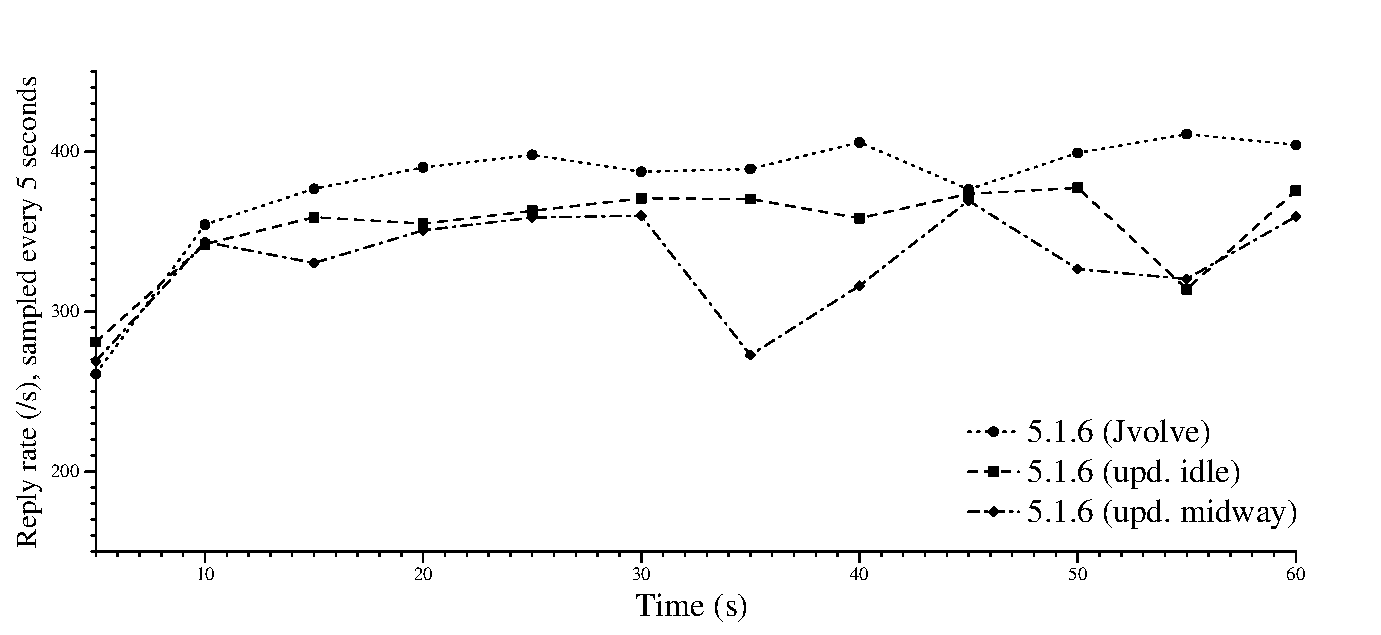
\includegraphics[width=0.5\textwidth]{jetty}
\caption{Webserver request rate over time\label{fig:jetty}}
\label{fig:jetty-rate}
\end{center}
\end{figure}

\subsection{Microbenchmarks}
\label{subsec:microbench}

The two factors that determine \DSU{} update time are the time to
perform a GC, determined by the number of objects, and the time to run
object transformers, determined by the fraction of objects being
updated. To measure the costs of each, we devised a simple
microbenchmark that creates objects and transforms a specified
fraction of these objects when a \DSU{} update is triggered. The
microbenchmark has two simple classes, \texttt{Change} and
\texttt{NoChange}.  Both start with a single integer field.  The
update adds another integer field to \texttt{Change}.  The
user-provided object transformation function copies the first field and
initializes the new field to zero.  The benchmark contains two arrays,
one for \texttt{Change} objects and one for \texttt{NoChange} objects.
We measure the cost of performing an update while varying the total
number of objects and the fraction of objects of each type.

Table~\ref{tab:microbench} shows the \DSU{} pause time for 1000 to 100000
objects (the rows) while varying the fraction of the objects that are of
type \texttt{Change} (the columns).  The first group of rows measures the
total pause time, the second group measures the portion of this time due to
running transformer functions, and the final group measures the portion of
this time due to running the garbage collector.  The first column of the
table shows that there is large fixed cost of performing a whole heap
collection even for a small number of objects.  This time includes the time
to stop the running threads and perform other setup.  As we move right in
the table, we can see that the cost of object transformation can outweigh
the cost of the garbage collection by quite a bit. Also, with more objects
to be transformed, the time to run object transformation functions
increases non-linearly, because of caching effects.

The highly optimized original copying sequence does a \texttt{memcopy}, whereas
our transformer functions use reflection and copy one field at a time.
For each transformed object, \DSU{} looks up and invokes an object's
\texttt{jvolve\_object} function using reflection, and then copies
each of the fields one by one.  The cost of reflection could be
reduced by caching the lookup, but a na\"ively compiled field-by-field
copy is much slower than the collector's highly-optimized copying loop.
Note however that the number of transformed objects in our actual
benchmarks was usually very low, less than 25 objects in the
applications we considered, as illustrated by Jetty pause times reported
above.

% \begin{verbatim}
% Total DSU Pause
%               0.00    0.10    0.20    0.30    0.40    0.50    0.60    0.70    0.80    0.90    1.00
%       1000  538.96  540.57  587.53  554.98  552.78  550.44  561.87  557.66  564.31  567.02  773.40
%      10000  529.42  584.29  597.35  624.16  647.52  675.41  721.26  738.99  811.14  773.39  799.17
%      50000  379.79  462.63  542.68  622.79  702.85  785.25  867.00 1536.62 1779.80 2020.53    None
%     100000  377.46  588.79  703.45  862.07 1777.40    None    None    None    None    None    None
%     500000  380.02 2468.65    None    None    None    None    None    None    None    None    None
%    1000000  405.53    None    None    None    None    None    None    None    None    None    None
% 
% Running transformation functions
%               0.00    0.10    0.20    0.30    0.40    0.50    0.60    0.70    0.80    0.90    1.00
%       1000    0.24    2.29    3.93    5.05    6.60    7.72    8.95   10.47   11.78   13.15   19.92
%      10000    0.24   14.64   28.45   42.66   58.38   70.13   84.34  109.72  114.00  125.96  140.16
%      50000    0.18   43.92   87.46  132.97  177.81  220.91  263.90  901.65 1108.51 1312.36    None
%     100000    0.18   96.34  175.59  262.64 1106.61    None    None    None    None    None    None
%     500000    0.17 1649.37    None    None    None    None    None    None    None    None    None
%    1000000    0.17    None    None    None    None    None    None    None    None    None    None
% 
% Garbage collection
%               0.00    0.10    0.20    0.30    0.40    0.50    0.60    0.70    0.80    0.90    1.00
%       1000  535.50  531.06  575.74  542.62  538.93  535.42  545.64  540.06  545.20  546.65  743.59
%      10000  525.84  562.48  561.50  574.23  581.97  598.06  629.68  622.11  689.90  640.29  651.72
%      50000  377.46  414.06  450.64  485.18  520.44  559.70  598.41  630.29  666.66  703.40    None
%     100000  375.16  487.49  523.03  594.53  665.91    None    None    None    None    None    None
%     500000  377.71  813.98    None    None    None    None    None    None    None    None    None
%    1000000  403.19    None    None    None    None    None    None    None    None    None    None
% \end{verbatim}

% \begin{verbatim}
% Jetty-5.1.10 - 5 January 2006
% slloccount: 44102 lines
%  + Fixed path aliasing with // on windows.
%  + Fix for AJP13 with multiple headers
%  + Fix for AJP13 with encoded path
%  + Remove null dispatch attributes from getAttributeNames
%  + Put POST content default back to iso_8859_1. GET is UTF-8 still
% 
% Jetty-5.1.9 - 7 December 2005
% slloccount: 44084 lines
%  + Fixed wantClientAuth(false) overriding netClientAuth(true) 
% 
% Jetty-5.1.8 - 7 December 2005
% slloccount: 44082 lines
%  + Fixed space in URL issued created in 5.1.6
% 
% Jetty-5.1.7 - 7 December 2005
% slloccount: 44081 lines
%  + Improved collection of statistics
%  + Better support for requst encoding.
% 
% Jetty-5.1.6 - 18 November 2005
% slloccount: 43948 lines
%  + Fixed JSP visibility security issue.
%  + Improved jetty-web.xml access to org.mortbay classes.
% 
% Jetty-5.1.5 - 10 November 2005
% slloccount: 44027 lines
%  + Improved shutdown hook
%  + Improved URL Decoding
%  + Improved mapping of JSP files.
% 
% Jetty-5.1.4 - 5 June 2005
% slloccount: 43578 lines
%  + Fixed FTP close issue.
%  + setup MX4J with JDK1.5 in start.config
%  + set classloader during webapp doStop
%  + NPE protection in ThreadedServer
%  + ModelMBean handles null signatures
%  + Change JAAS impl to be more flexible on finding roles
% 
% Jetty-5.1.3 - 7 April 2005
% slloccount: 43612 lines
%  + Some minor code janitorial services
% 
% Jetty-5.1.2 - 18 January 2005
% slloccount: 43277 lines
%  + Added id and ref support to XmlConfiguration
%  + Cleaned up AbstractSessionManager synchronization.
%  + Fixed potential concurrent login problem with JAAS
%  + Apply patch #1103953
% 
% Jetty-5.1.1 - 1 December 2004
% slloccount: 43073 lines
%  + Changes to key pair handling for SSL.
% 
% Jetty-5.1.0 - 14 November 2004
% slloccount: 42981 lines
% \end{verbatim}

% vim:ft=tex:spell:


\section{Plan and proposed schedule}
\label{sec:schedule}

This section describes the current status of our work and our plan for the
future.

\paragraph{Status}
\begin{itemize}
\item We have a proof-of-concept implementation that demonstrates \acf{DSU} for
Java by supporting two years worth of updates to three server applications.
This submission is currently under review.
\end{itemize}
\paragraph{Plan}
\begin{itemize}
\item We are in the early stages of modifying \acf{OSR} to support
\acs{DSU}. We plan to have an implementation by middle of September 2008.
We will then work on making the implementation more robust with a better \acf{UPT};
\DSU{} running on multiprocessors; and better analysis of applications and
performance. We intend to have a submission to PLDI 2009 (deadline:
November 2008).
\item Starting September 2008, we will begin exploring other object
transformation models; starting with 1) running object transformation
functions within the collector while copying objects, and then moving on to
2) supporting DSU in a concurrent collector (January 2009 - May 2009).
\item We intend to examine more applications during Summer 2009, spend Fall
writing the dissertation, with an expected graduation date in the Fall of
2009.
\end{itemize}

\section{Conclusions}
\label{sec:conc}

This paper presents \DSU, a Java virtual machine with support for
dynamic software updating.  \DSU{} is the most full-featured,
best-performing implementation of DSU for Java published to date.  We
demonstrate its flexibility and safety by successfully applying updates
for one to two years worth of releases for three programs: Jetty
webserver, JavaEmailServer, and CrossFTP server.  \DSU{} imposes no
overhead during a program's steady-state  execution.  
\DSU's DSU support builds naturally
on top of existing VM services, including dynamic class loading,
thread synchronization, return barriers, on-stack replacement, JIT compilation, and
garbage collection.  It is probably optimistic to believe that DSU
will be able to support every update.  Nevertheless, our results
demonstrate that dynamic software updating support can be naturally
incorporated into modern VMs, and that doing so has the potential to
significantly improve software availability by reducing downtime.


\begin{small}
\bibliographystyle{plain}
\bibliography{paper}
\end{small}


\acrodef{DSU}{Dynamic software updating}
\acrodef{UPT}{Update Preparation Tool}
\acrodef{OSR}{On-Stack Replacement}
\acrodef{JIT}{Just-in-time}
\acrodef{GC}{Garbage Collection}


\end{document}
